\begin{refsection}
\chapter{Multi-ion Effects and Na$^+$ Selectivity over K$^+$ in Sodium Channel Na\textsubscript{V}Ab}

Contributions by Christopher Ing (CI) and Regis Pomes (RP): C.I. and R.P. designed the research. Simulations were performed by C.I. Data analysis was performed by C.I. and R.P. The manuscript was written by R.P. and C.I.

\newpage

\section{Summary}

The structural determination of the prokaryotic voltage-gated sodium channel Na\textsubscript{V}Ab has enabled the elucidation of the molecular determinants of cation permeation and selectivity.  To examine the microscopic basis for selectivity of Na\textsubscript{V}Ab for Na$^+$ over K$^+$, we generated dozens of 1000-ns molecular dynamics trajectories in the presence of NaCl, KCl, or a mixture of the two. Na$^+$ and K$^+$ bind in similar ways in the selectivity filter of Na\textsubscript{V}Ab, with multiple binding modes involving a variable number of cations and flexible E177 side chains. Na$^+$ movement through the selectivity filter is coupled to the conformational isomerization of E177 between out-facing and lumen-facing rotamers. Na$^+$ conduction proceeds through a loosely-coupled knock-on mechanism involving an interconversion between 2 and 3 bound ions within the selectivity filter, lowering the free energy for Na$^+$ conduction. K$^+$ conduction proceeds through a single-file knock-on mechanism with relatively static binding sites. In mixed cation simulations, Na$^+$ is favored over K$^+$ at primary binding sites by a factor of 2-3. Modifications to the EEEE ring of the selectivity filter with artificial conformational restraints, the E177D mutation, or E177 protonation, dramatically alter selectivity, supporting E177 as a critical determinant for Na$^+$ selectivity in bacterial Nav channels.

\section{Introduction}

Ion channels of excitable cells can be highly selective, but the structural basis of selectivity remains unclear \cite{Hille:2001tw}.   Based on the crystal structure of the K$^+$ channel KcsA \cite{Doyle:1998wq}, the 104-fold  preference of that channel for K$^+$ over Na$^+$ was first explained by invoking the snug-fit model \cite{Bezanilla:1972uz}, in which the selectivity filter (SF) of the channel is essentially rigid.  However, molecular dynamics (MD) simulations of KcsA \cite{Guidoni:1999ba} subsequently showed that the SF of KcsA is flexible \cite{Andersen:2011ty}, igniting a debate on the role of structural fluctuations of the protein in ionic selectivity.  Various theoretical models have been employed in the past decade in an effort to elucidate the molecular determinants for the selectivity of K$^+$ over Na$^+$ in KcsA, emphasizing the balance of ion-channel and channel-channel interactions \cite{Noskov:2004tv} as well as the spatial constraints imposed on the SF by the protein fold \cite{Andersen:2011ty,Bostick:2010bm,Dixit:2011wf,Roux:2011ed,Varma:2011gn}. The role of both equilibrium and kinetic factors in selectivity is thought to be essential for the NaK channel, based on electrophysiological measurements of two single-point mutants, one of which was found to be selective and the other non-selective despite both channels being reported as K$^+$ selective over Na$^+$ at equilibrium on the basis of isothermal titration calorimetry and crystallographic titration \cite{Liu:2013hf,Sauer:2013gk}. 

While the molecular basis of ionic selectivity in K$^+$ channels is still under debate, even less is known about Na$^+$ selectivity.  The recent elucidation of the structures of bacterial voltage-gated Na$^+$ channels Na\textsubscript{V}Ab \cite{Payandeh:2012ib,Payandeh:2013ex}, NavMs \cite{McCusker:2012di} NavAep1 \cite{Shaya:2014gg}, and NavRh \cite{Zhang:2013bz} provides a structural basis for answering that question. The molecular structure of the SF of Na\textsubscript{V}Ab (TLESW) is both wider and shorter than that of K$^+$ channels such as KcsA (TVGYG).  In KcsA, channel coordination of permeating cations consists entirely of direct interactions with backbone carbonyl oxygen atoms, whereas in Na\textsubscript{V}Ab, the SF is lined with amino acid side chains from S178 and E177 in addition to backbone carbonyl groups from T175 and L176 \cite{Doyle:1998wq,Payandeh:2012ib,Jiang:2003vh}.  Due to the tetrameric domain arrangement of Na\textsubscript{V}Ab, the E177 site forms a ring of four glutamate side chains (EEEE) in the same sequence positions as the characteristic DEKA ring of eukaryotic sodium channels \cite{Heinemann:1992ep,Terlau:1991ud}. Simulation studies have revealed that dynamic fluctuations of these four glutamic acid side chains can effectively modulate the diameter of the SF as ions bind and diffuse through it \cite{Boiteux:2014ut,Chakrabarti:2013kd}. In contrast with strongly selective K$^+$ channels, this raises the question of how a wider and more flexible SF could result in a weakly selective channel, on the order of 10:1 for Na$^+$ over K$^+$ \cite{Payandeh:2012ex,Ulmschneider:2013da}. 

Recent MD studies have examined the conduction of Na$^+$ and K$^+$ in bacterial voltage-gated Na$^+$ channels \cite{Boiteux:2014ut,Corry:2012ge,Domene:2015kj, FinolUrdaneta:2014bz,Furini:2012jl,Ngo:2016es,Ulmschneider:2013da,Chakrabarti:2013kd}. Na$^+$ conduction was found to occur through a loosely coupled knock-on mechanism, whereby an incoming Na$^+$ causes an ion bound within the SF to move into the central cavity (CC), but wherein the movement of both ions are not necessarily concerted. Unbiased and biased sampling techniques have been used to compute the lowest free-energy conduction pathway for multiple Na$^+$ or K$^+$ within the SF, identifying regions within the SF that were selective. Across several of these studies, Na$^+$ and K$^+$ were found to bind at similar sites within the SF, with different relative affinities \cite{Ing:2016em}. In a study utilizing unbiased non-equilibrium simulations \cite{Ulmschneider:2013da}, the computed Na$^+$:K$^+$ selectivity, based on a ratio of conductance, was found to be in agreement with experimental values. However, no study has described a molecular mechanism for Na$^+$ selectivity involving three ion occupancy of the SF, nor has such a mechanism been described on the basis of unbiased equilibrium studies at physiological voltages. 

Among the previous Nav channel studies, our analysis showed that E177 side chains are essential ligands of Na$^+$ and that their conformational isomerization is coupled to binding and movement of Na$^+$ \cite{Chakrabarti:2013kd}. Multiple studies have since analyzed the role of glutamic acid sidechain fluctuations in Na$^+$ conduction \cite{Boiteux:2014ut,Domene:2015kj,Furini:2014gv,Ke:2014fy}. A similar mechanism has been discovered in the glutamate ring of the cation-selective nicotinic acetylcholine receptor \cite{Harpole:2014gu}. These findings raise the question of the role of Glu binding and dynamics in ion selectivity of Na\textsubscript{V}Ab and other Na$^+$-selective channels. Experimental measurements reveal that both the side-chain shortening mutation E177D and lowering the pH can modulate Na$^+$ over K$^+$ selectivity in the channel NaChBac \cite{FinolUrdaneta:2014bz}. In the experiments presented here, we follow up our previous studies of Na$^+$ permeation in Na\textsubscript{V}Ab \cite{Chakrabarti:2013kd} with experiments on K$^+$ permeation in isolation and on Na$^+$ and K$^+$ permeation in competition with each other. We compare permeation in four closed-channel systems; the wildtype (WT) channel, WT with conformational restraints on the E177 side chain, the E177D mutant, and WT with a single protonated E177 side chain. In order to examine the reversible diffusion of ions in and out of the SF, as well as competitive binding, we generated ten to twenty 1000-ns trajectories for each system in the presence of NaCl, KCl, and a mixture of the two, for a total sampling time of 200 $\mu$s. To test the generality of our findings and to understand the extent to which systematic errors can alter ion binding properties, we repeated NaCl and KCl simulations using the WT channel system with four alternate force fields. Across several force fields, our results show that selectivity emerges due to a dynamic fluctuations of the SF favoring Na$^+$ over K$^+$. A loosely-coupled knock-on mechanism, facilitated by E177 side chains, results in a diffusive energy landscape for Na$^+$ but not for K$^+$, manifesting as a selective advantage for Na$^+$ in mixed cation simulations. 

\section{Results}

\subsection{Na$^+$ and K$^+$ Ions in the Na\textsubscript{V}Ab Pore}

\begin{figure}[!ptb]
\centering\
\includegraphics[width=0.8\textwidth]{nav2/Nav2Fig1}
\caption[Sodium and potassium ion movement in the selectivity filter of Na\textsubscript{V}Ab]{\textbf{Sodium and potassium ion movement in the selectivity filter of Na\textsubscript{V}Ab}. (\textbf{A}) Representative snapshots of Na$^+$ and K$^+$ (spheres) in the SF sampled from two time trajectories.  Ions are colored red, green, and blue from the bottom (intracellular end) to the top (extracellular) in the channel.  The pore-lining oxygen groups of the SF (backbone carbonyl groups of T175 and L176 and the side chains of E177 and S178) are shown. Water molecules are not shown.  (\textbf{B, D}) Movement of Na$^+$ or K$^+$ cations along the pore axis from selected simulation repeats. (\textbf{C, E}) Distribution of Na$^+$ or K$^+$ along the pore axis over all simulation repeats, with colored sub-distributions representing the coordination groups of a permeating ion at that axial position. Colored bars at the bottom of time series (\textbf{B}) and (\textbf{D}) indicate the channel occupancy state (legend in top right).}
\label{fig:nav2fig1}
\end{figure}

Figure \ref{fig:nav2fig1} depicts two MD time trajectories obtained in presence of either NaCl (Fig. \ref{fig:nav2fig1} B) or KCl (Fig. \ref{fig:nav2fig1} D) in the closed state of Na\textsubscript{V}Ab (PD+VSD model, pore domain and voltage sensors, Fig. \ref{fig:nav2figS1}). Molecular renderings at different time points show that ions occupying the SF can be coordinated to a variable number of glutamic acid side chains (Fig. \ref{fig:nav2fig1} A). We observe reversible diffusion of Na$^+$ and K$^+$ in and out of the SF, with total channel occupancy that fluctuates between two (Fig. \ref{fig:nav2fig1} A i,v) and three ions (Fig. \ref{fig:nav2fig1} A ii-iv), labelled along the time trajectories by yellow and purple bars, respectively (Fig. \ref{fig:nav2fig1} B,D). In the three ion occupancy state, two Na$^+$ may reside at nearly the same axial position ($\sim$850 ns in Fig. \ref{fig:nav2fig1} B), but K$^+$ did not adopt this configuration, remaining in a single-file arrangement. At several points along the time trajectory, regardless of the total channel occupancy, the innermost ion (in red) moves in and out of the central cavity (CC). Sequential movement of Na$^+$ or K$^+$ may occur through a concerted knock-on mechanism, whereby an outer ion displaces the innermost ion into the CC ($\sim$650 ns for Na$^+$, $\sim$350 ns for K$^+$, in Fig. \ref{fig:nav2fig1} B,D, respectively). Similarly, ion permeation may also occur through a loosely-coupled knock-on mechanism, whereby the innermost ion enters the CC without requiring the entry of a new ion into the SF ($\sim$860 ns for Na$^+$, $\sim$750 ns for K$^+$ in Fig. \ref{fig:nav2fig1} B,D, respectively). 

\begin{figure}[!ptb]
\centering
\includegraphics[width=0.7\textwidth]{nav2/Nav2FigS4}
\caption[Binding modes of Na$^+$ or K$^+$ along the pore axis]{\textbf{Binding modes of Na$^+$ or K$^+$ along the pore axis}. Total ionic distributions are shown for Na$^+$ (blue solid line; left half panel) and K$^+$ (green solid line; right half panel) with colored sub-distributions identifying the groups of channel oxygens coordinating an ion at that axial position. Binding modes are defined by coordination to one or more channel ligands in either the first or second coordination shell (S178-only, E177-only, E177 and L176, L176 and T175, or no coordination in the central cavity). A gold band indicates the region of highest free-energy barrier for K$^+$ permeation within the SF. Distributions are normalized by channel average channel occupancy.}
\label{fig:nav2figS4}
\end{figure}

The axial distribution of ion positions averaged across all simulation repeats indicates that Na$^+$ and K$^+$ differ in E177 (`E') and combined E177/L176 (`EL') coordination, but share a very similar L176/T175 (`LT') binding site (Fig. \ref{fig:nav2fig1} C,E). The distribution of ions in the `E' and `EL' binding modes are broad and strongly overlap for Na$^+$ but not for K$^+$, which is sharply localized at non-overlapping sites. Similar features are observed in a pore-domain only (PD model) with pure NaCl or KCl solutions (Fig. \ref{fig:nav2figS4} C). The average occupancy of the pore is similar across all pure-NaCl and pure-KCl simulations ($2.2 \pm 0.1$ for Na$^+$ and $2.5 \pm 0.1$ for K$^+$, Fig. \ref{fig:nav2fig2} B). The most significant difference between the two solutions is that two Na$^+$ cations occupy the `EL' binding site in $11.33 \pm 0.04$\% frames. Although a large number of ionic arrangements were sampled within the SF, dual ion occupancy of the `EL' site occurs most frequently in conjunction with single occupancy of the `E' site (Figs. \ref{fig:nav2fig1} A iii, \ref{fig:nav2fig2} C).  The most populated ionic arrangements of NaCl and KCl simulations, accounting for 84.1\% and 89.2\% of frames, respectively, suggest that the two cations differ in that the SF can accommodate multiple Na$^+$ at similar axial positions near the `E' and `EL' sites, but that K$^+$ must traverse the SF in a single-file arrangement. 

\begin{figure}[!ptb]
\centering
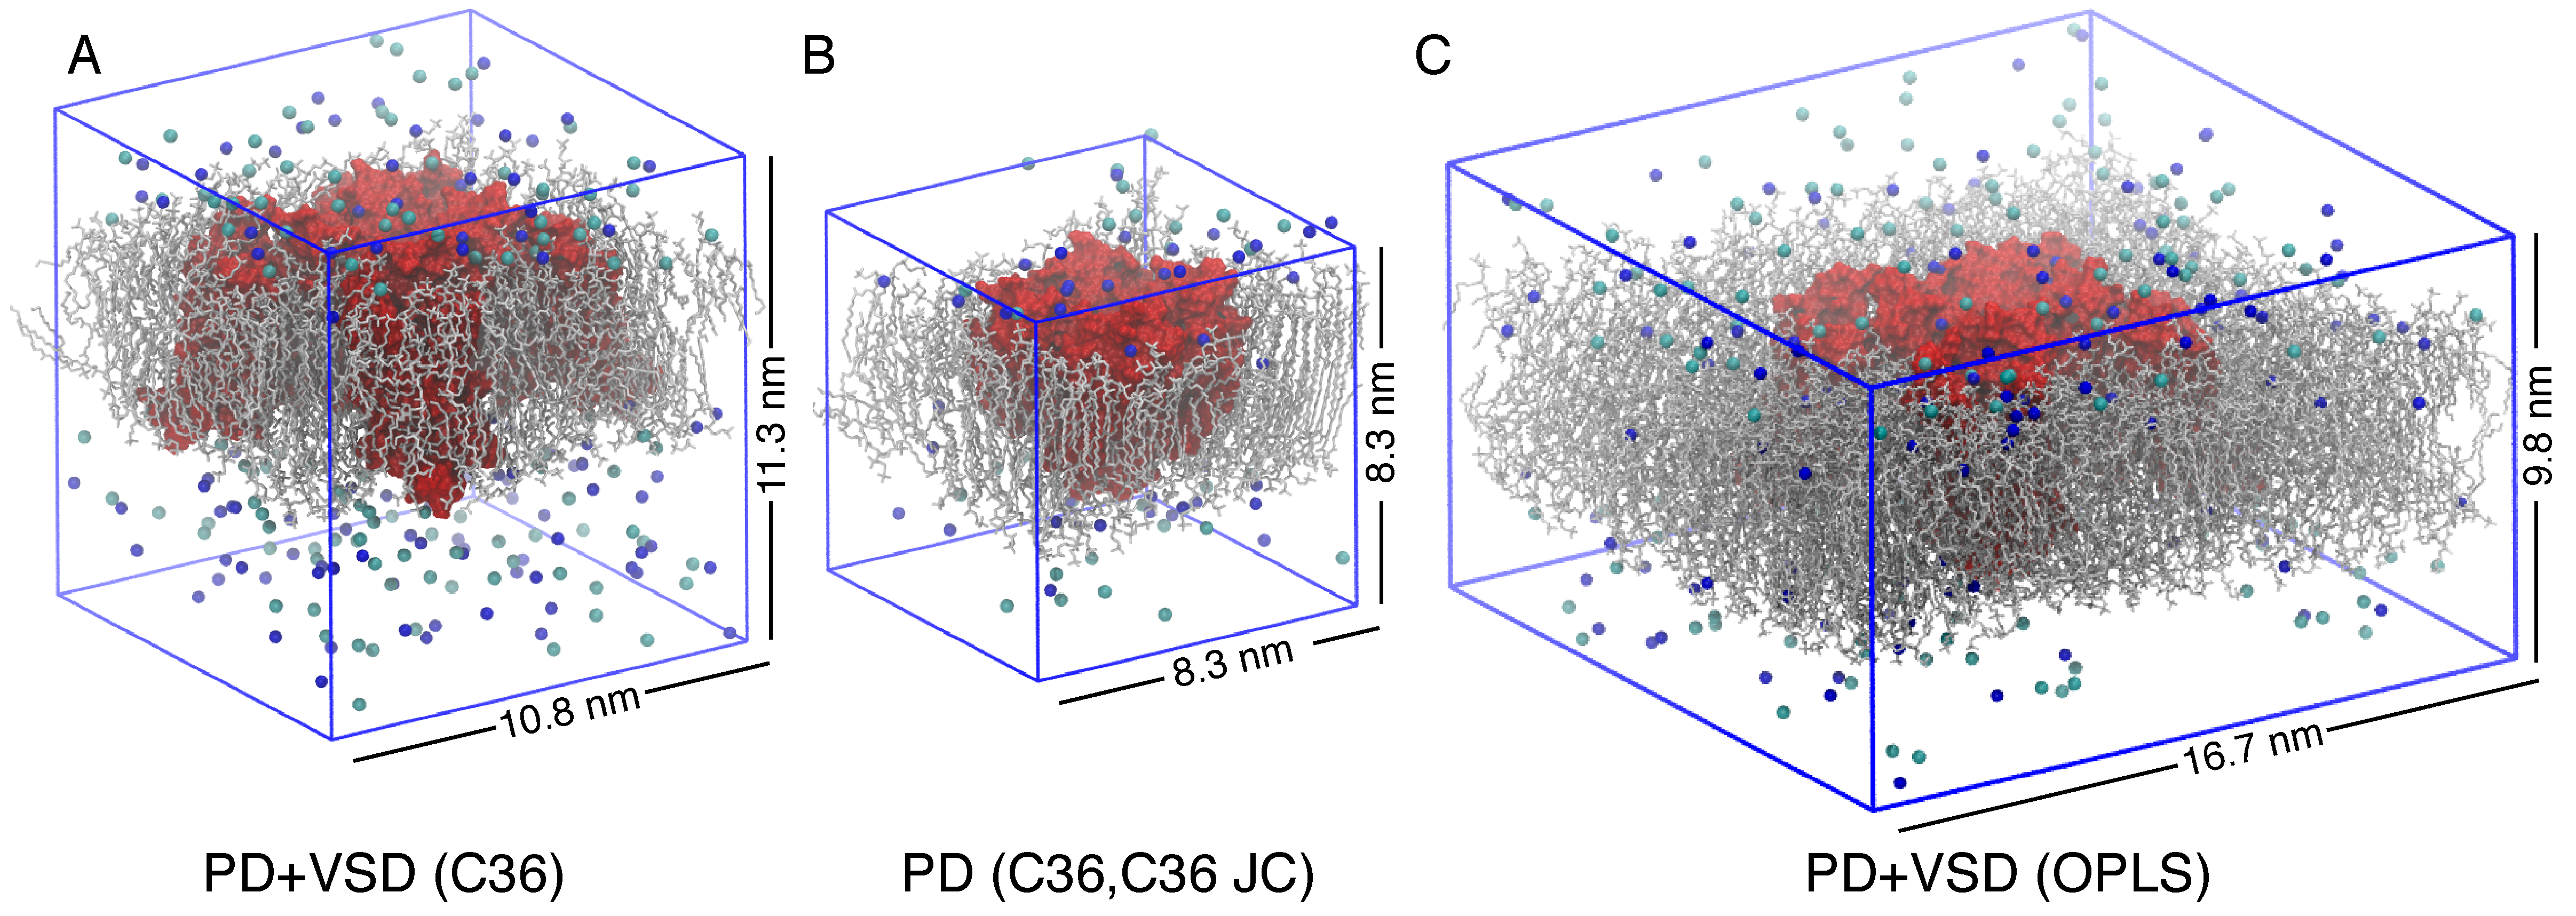
\includegraphics[width=0.9\textwidth]{nav2/Nav2FigS1}
\caption[Molecular models of Na\textsubscript{V}Ab in a hydrated lipid bilayer]{\textbf{Molecular models of Na\textsubscript{V}Ab in a hydrated lipid bilayer}. Initial models of the (\textbf{A}) full channel including pore domain and voltage-sensing domains (PD+VSD), (\textbf{B}) pore domain-only model (PD) prepared for NaCl simulations, and (\textbf{C}) full channel with an alternate simulation force field (PD+VSD, OPLS). Na\textsubscript{V}Ab protein is rendered as a surface (red) with DMPC molecules shown in grey licorice representation. Na$^+$ and Cl- are shown as blue and aqua spheres, respectively, and water is not shown. }
\label{fig:nav2figS1}
\end{figure}

\subsection{Conformational Isomerization of Glu side chains}
In pure Na$^+$ and K$^+$ simulations, conformational isomerization of E177 side chains occurs spontaneously and reversibly. We have previously described how  Na$^+$ movement is coupled to the conformational isomerization of the side chains of E177, which is captured by dynamic changes in the number of conformationally flipped or `dunked' side chains \cite{Chakrabarti:2013kd}. Specifically, cation binding shifts the conformational equilibrium of E177 from the crystallographically-observed conformer, ($\chi_1$,$\chi_2$) = (t, g+), in which the carboxylate group points towards the EC mouth (Fig. \ref{fig:nav2fig2} A, yellow circle), to ($\chi_1$,$\chi_2$) = (t, g-), where the carboxylate group points into the lumen (Fig. \ref{fig:nav2fig2} A, purple circle) \cite{Chakrabarti:2013kd}.  An average of $2.1\pm 0.1$ and $2.0\pm  0.1$ carboxylate side chains adopt a lumen-facing conformation, for NaCl and KCl respectively. Isomerization of these side chains result in near charge compensation, directly coordinating an average of $2.0\pm0.1$ cations, for both NaCl and KCl (Fig. \ref{fig:nav2fig2} B). In the two time trajectories shown in Figure \ref{fig:nav2fig1}, the time series of the axial center of cationic and anionic charge have a Pearson correlation of YY and ZZ for Na$^+$ and K$^+$ simulations, respectively, indicating that Glu side chain dynamics is coupled to ion movement. 

\begin{figure}[!htb]
\centering
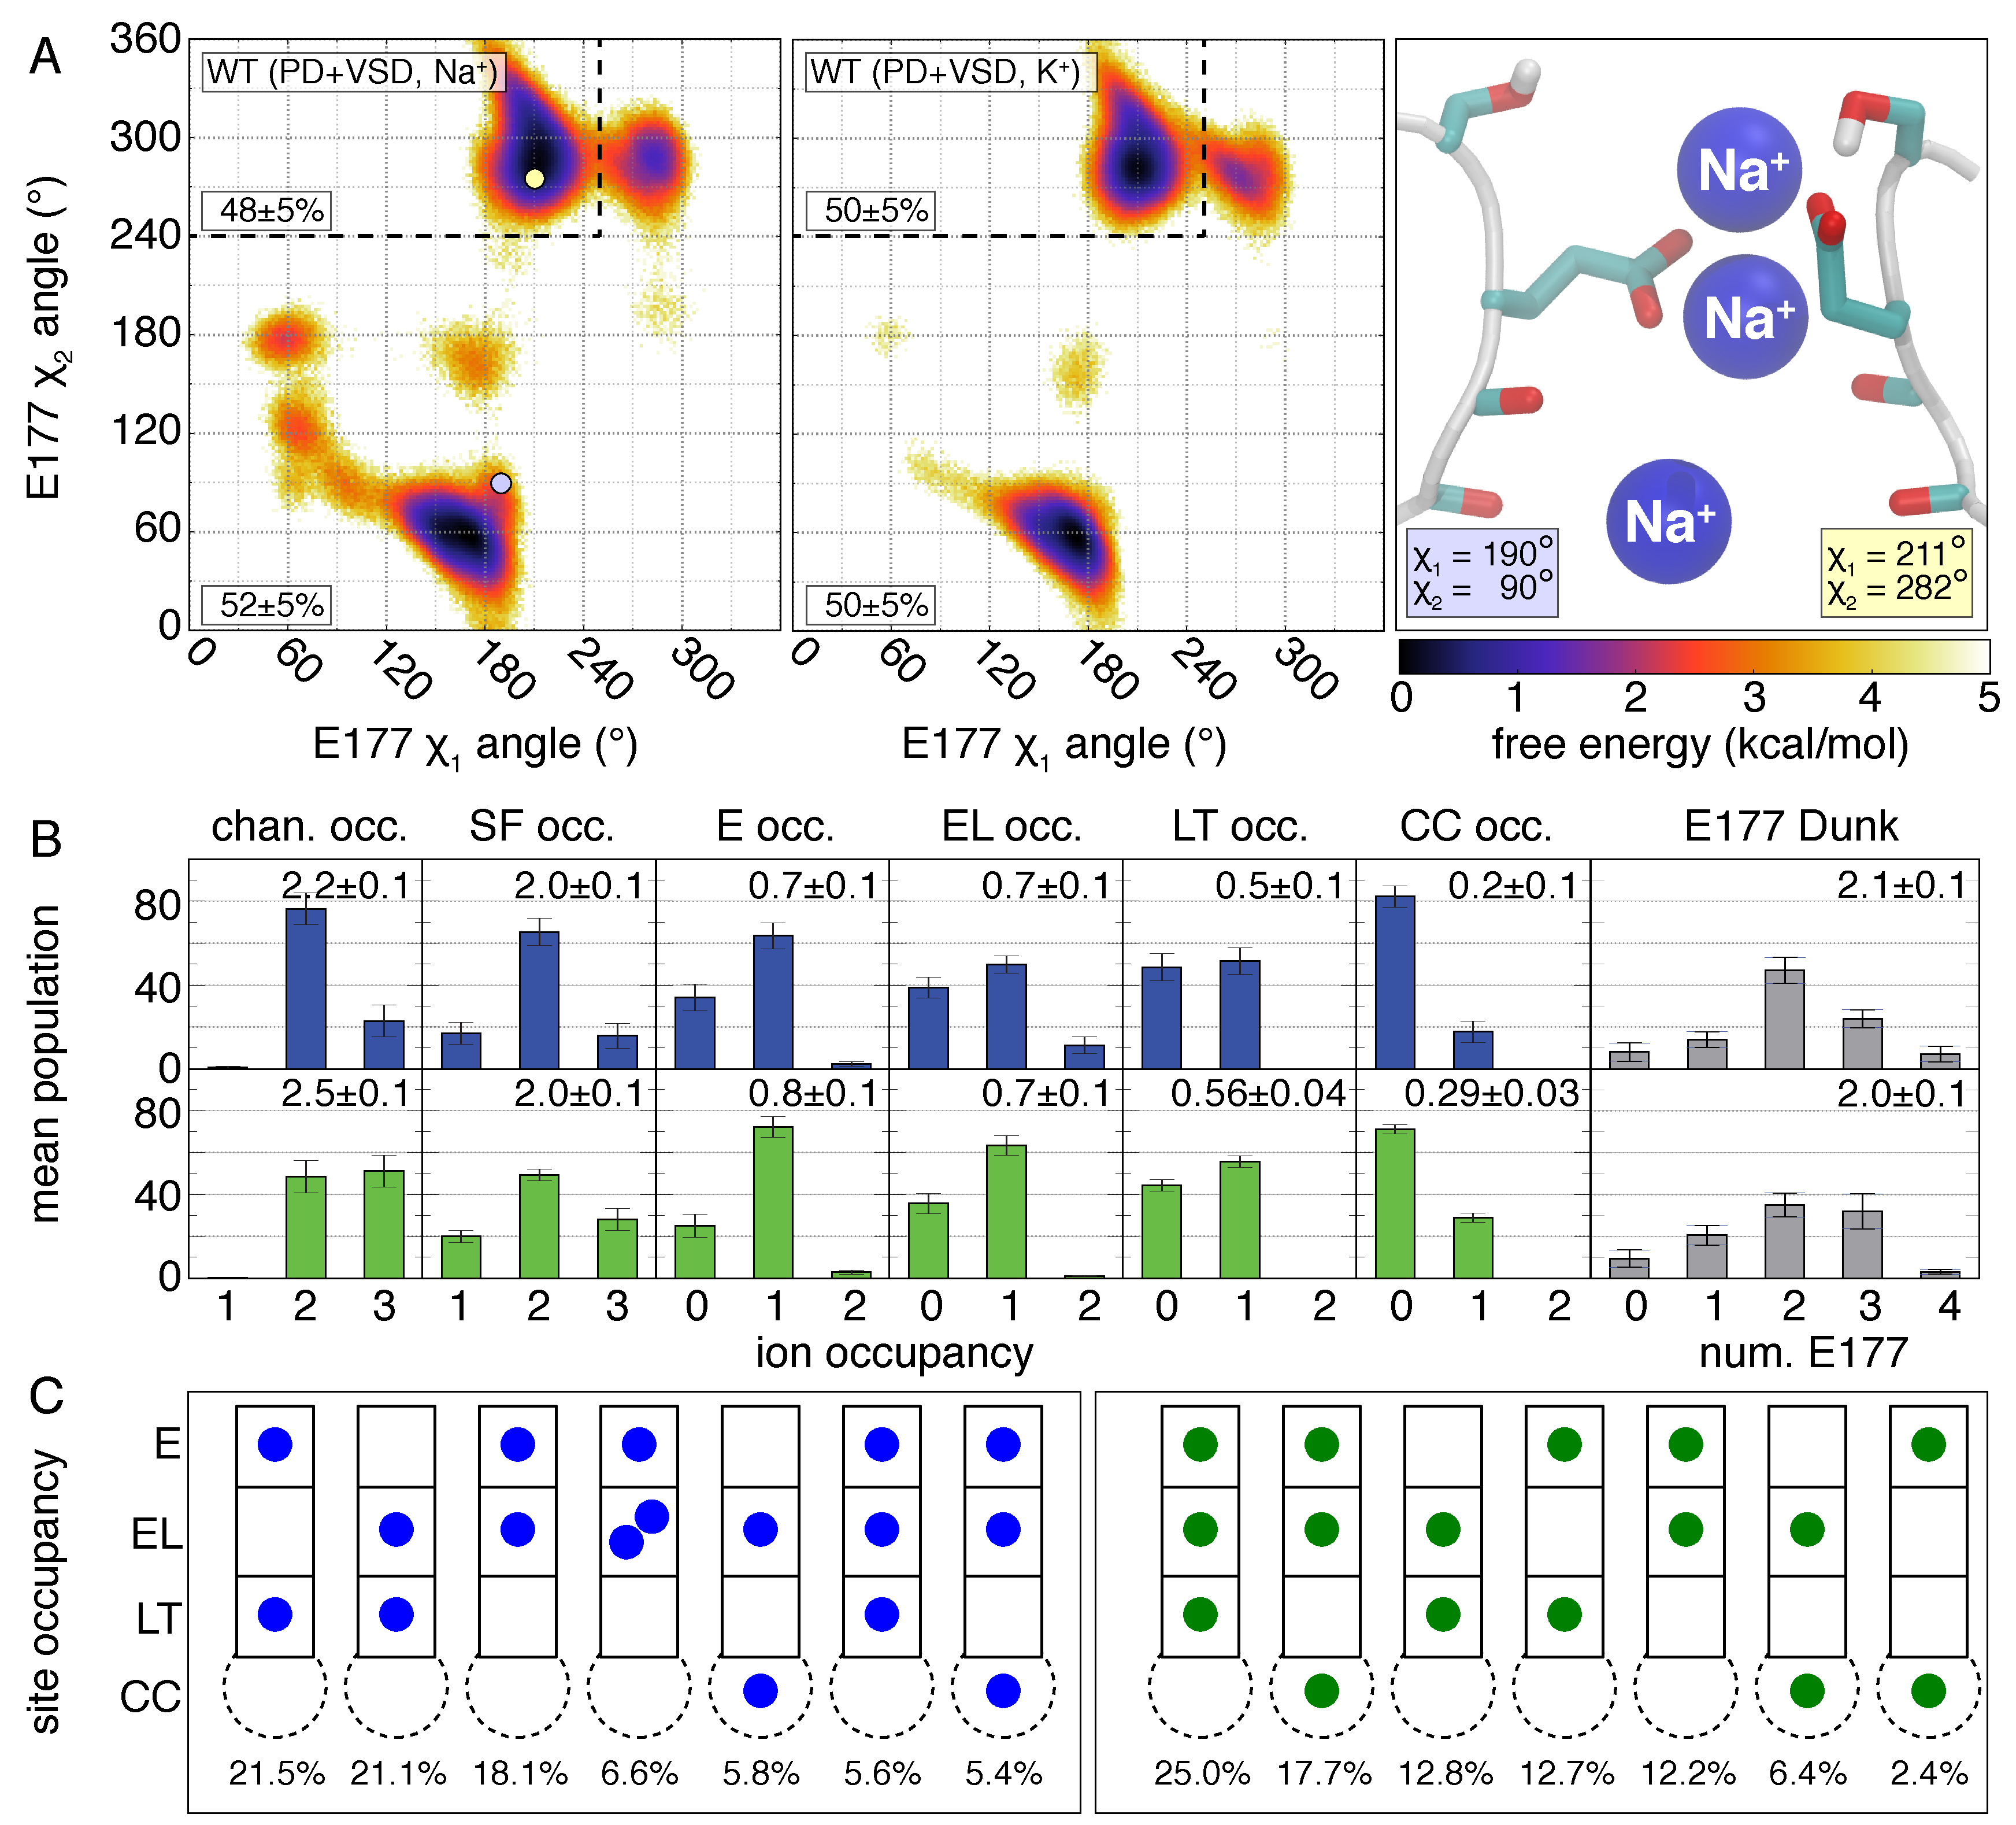
\includegraphics[width=0.7\textwidth]{nav2/Nav2Fig2}
\caption[Conformational isomerization of E177 side chains and ion binding statistics]{\textbf{Conformational isomerization of E177 side chains and ion binding statistics}. (\textbf{A}) Probability distribution of cation binding and E177 side-chain isomerization across all MD trajectories, for Na$^+$ (blue) and K$^+$ (green) in the PD+VSD model. (\textbf{A}) Free energy profiles for ($\chi_1$, $\chi_2$) of E177 in the PD+VSD model for pure Na$^+$ and K$^+$ ion concentrations, as well as pure Na$^+$ in the PD model with E177 dihedral restraints on all chains. Colored circles indicate the ($\chi_1$, $\chi_2$) value of the molecular rendering (right), and in-set boxes show the total percentage of data in two regions of $\chi_1$, $\chi_2$ space, corresponding to `undunked' and `dunked' conformations from top to bottom. (\textbf{B}) Ionic occupancy is shown from left to right for the entire channel, the SF, and for all major binding sites within the SF defined by 1st and 2nd shell coordination, together with the number of dunked E177 side chains. (\textbf{C}) Ionic occupancy of binding sites (E, EL, LT, CC) in the highest population channel configurations for pure Na$^+$ and K$^+$. Populations over all simulation repeats are shown below each state.}
\label{fig:nav2fig2}
\end{figure}

\subsection{Free Energy of Ion Permeation in the SF}

Two-dimensional potential of mean force (PMF) plots are shown for distinct ion pairs in order to identify the lowest free energy pathways for Na$^+$ and K$^+$ conduction (Fig. \ref{fig:nav2fig3}). Since dual occupancy of `EL' by Na$^+$ is dependent on the occupancy of the SF, free energy profiles are calculated separately for two (Fig. \ref{fig:nav2fig3} A-B) and three ion occupancies (Fig. \ref{fig:nav2fig3} C-H). The most populated channel occupancy state for both Na$^+$ and K$^+$, 2, involves the red and green ions adopting multiple configurations in the `E', `EL', and `LT' sites (Fig. 3A-B). For both Na$^+$ and K$^+$, the innermost ion (red), is primarily localized at the `LT' site ($\sim$4 \AA), but is capable of sampling a broad range of positions from 0 to $\sim$8 \AA. With two ions in the SF, the outermost ion (green) exchanges between the `E' and `EL' binding sites for both Na$^+$ and K$^+$, localized within the axial range of -4 to 0 \AA. However, a green Na$^+$ moves relatively unimpeded between `E' and `EL' binding sites, whereas a green K$^+$ resides at the `E' or `EL' sites, separated by a free energy barrier on the order of $\sim$1 kcal/mol. For both Na$^+$ and K$^+$, entry of the red ion into the CC occurs with highest propensity when the green ion holds a position near 0 \AA. 

\begin{figure}[hp]
\centering
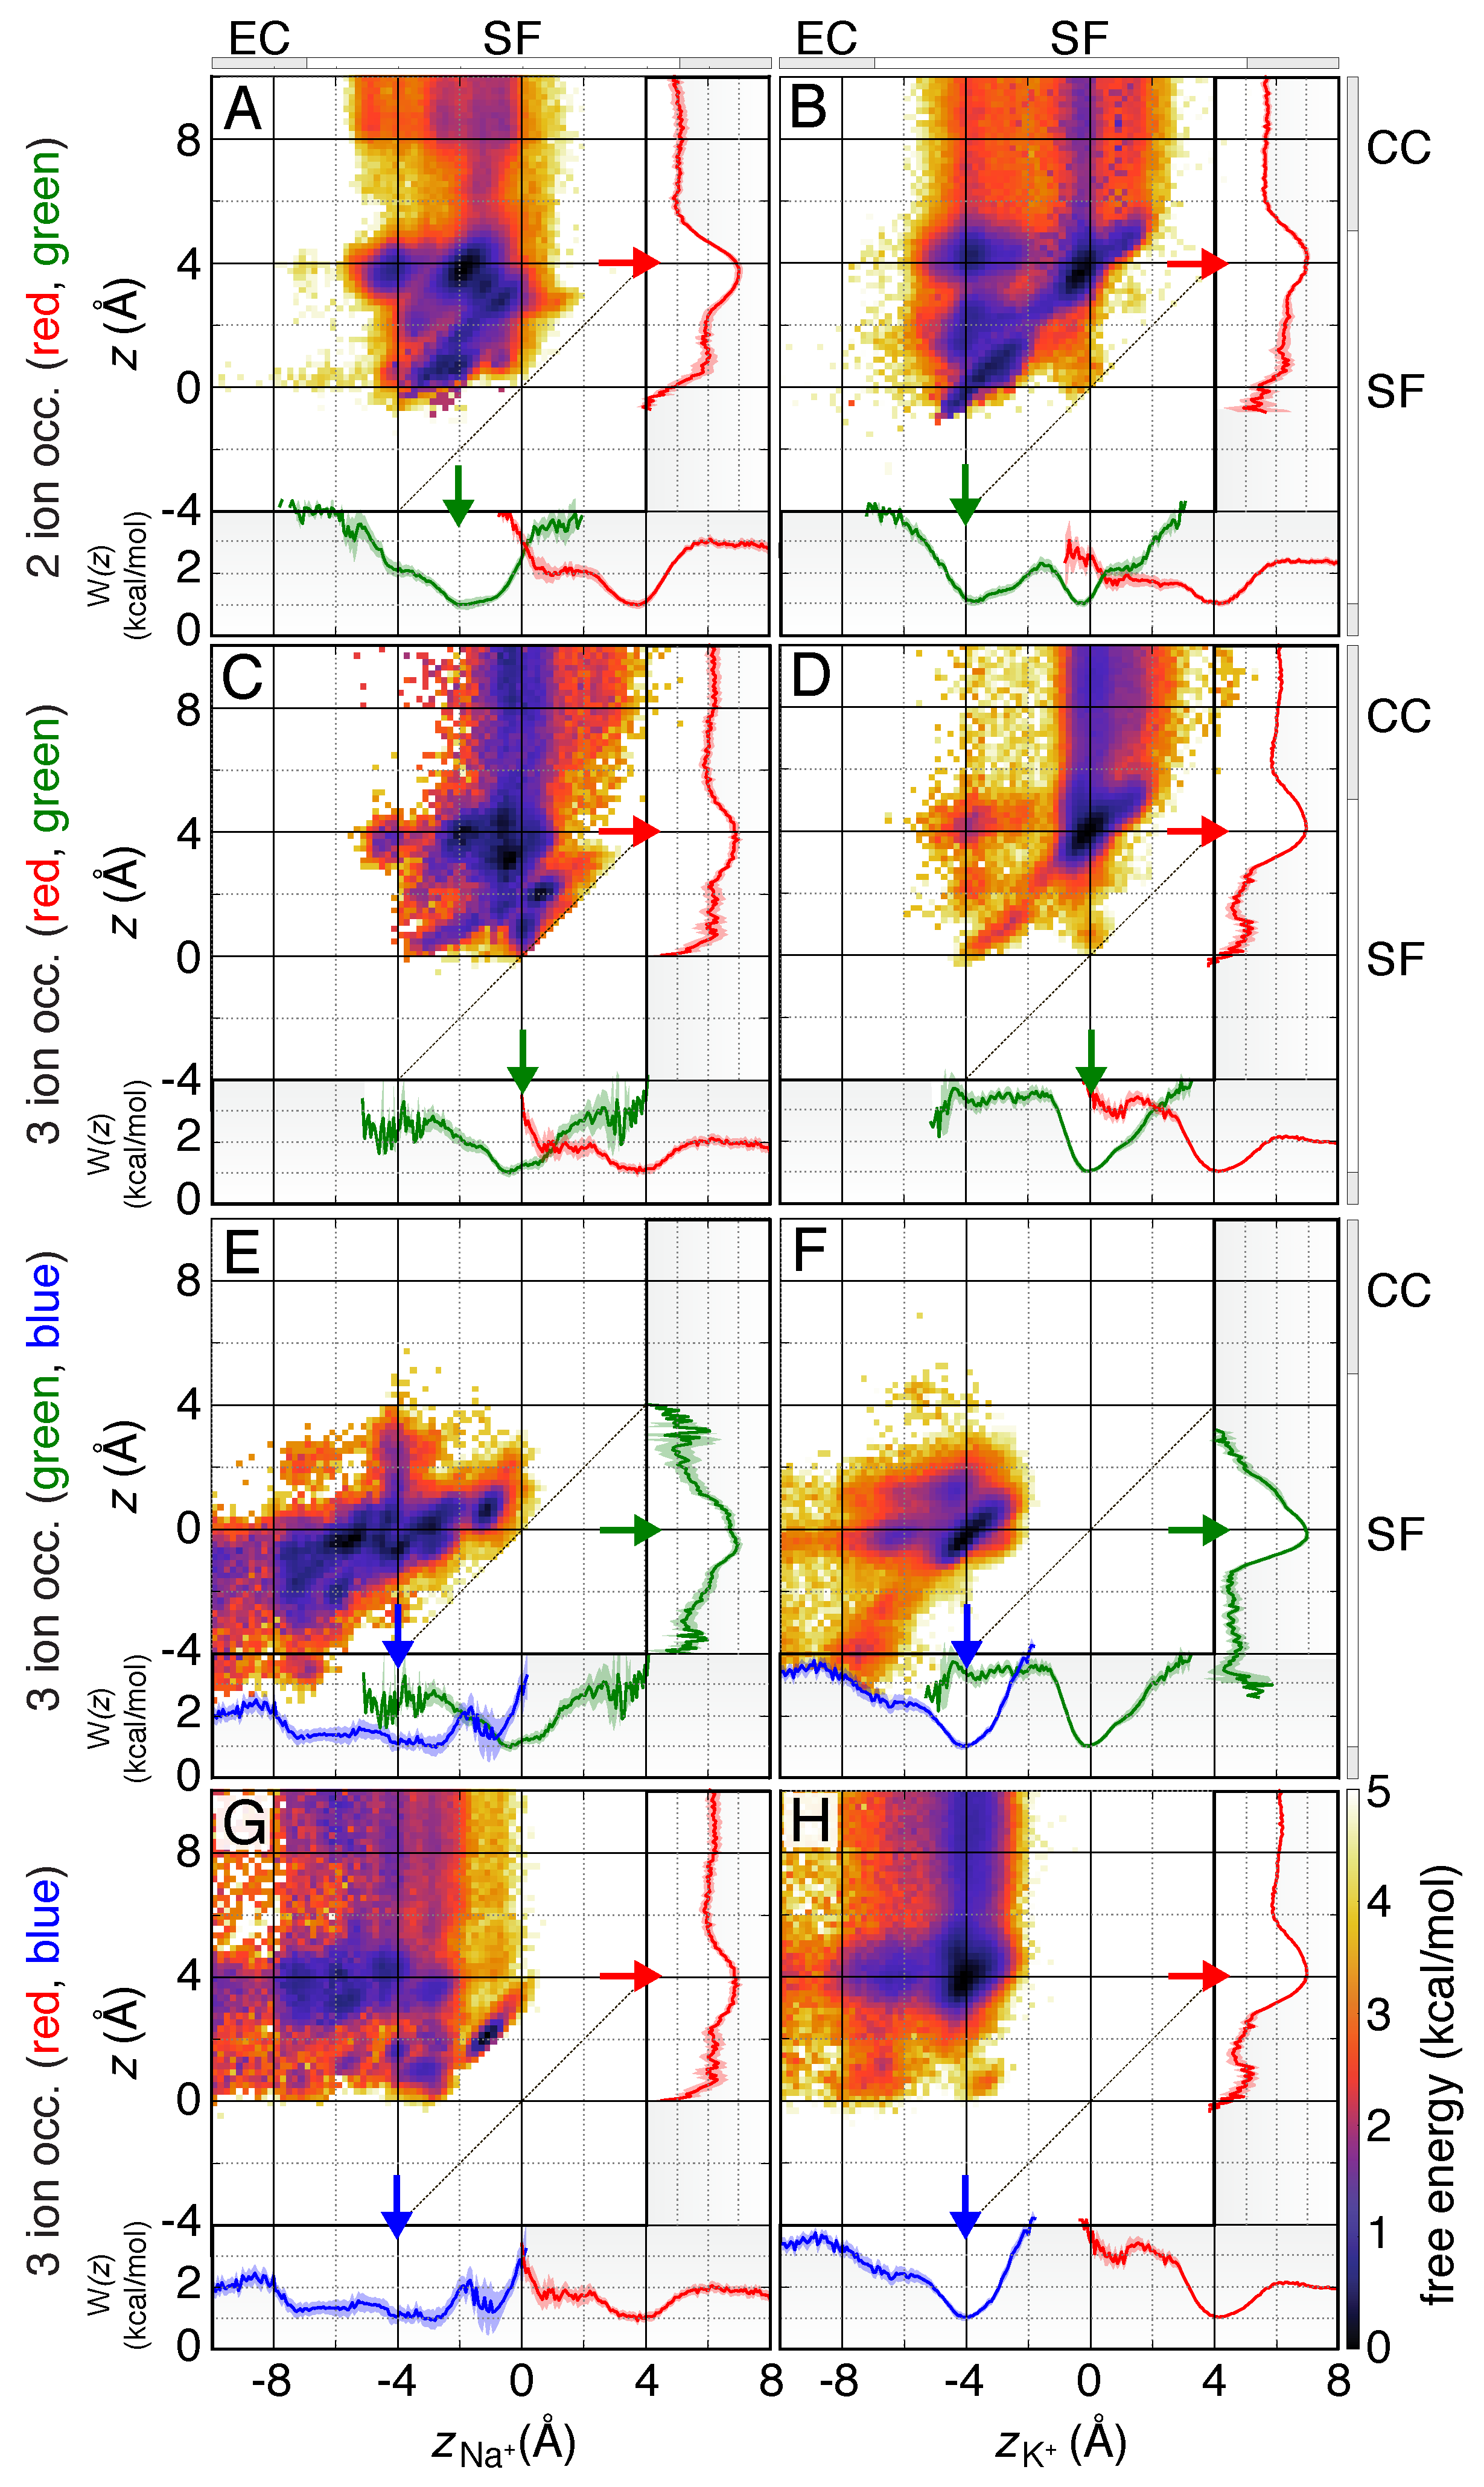
\includegraphics[width=0.6\textwidth]{nav2/Nav2Fig3}
\caption[Two-dimensional potential of mean-force (PMF) for Na$^+$ and K$^+$ pairs along the channel axis]{\textbf{Two-dimensional potential of mean-force (PMF) for Na$^+$ and K$^+$ pairs along the channel axis}. (\textbf{A}) Free energy landscape for (left) Na$^+$ and (right) K$^+$ pairs in the PD+VSD model. Ions are ranked by axial position from CC to EC with the colors `red', `green', and `blue' for both ion types. PMFs for Na$^+$ and K$^+$ are computed between ion pairs for channel occupancy states; (A, B) 2 and (C-H) 3. The populations of 2 and 3 ion states are 767 and 238\% for Na$^+$, respectively. For K$^+$, the populations are 488 and 518\% for 2 and 3 states respectively. One-dimensional projections of the axial free energy for each ion are shown on the vertical and horizontal axes and are colored for the target ion (identified with colored arrows). The reference state (zero free energy) of each panel is set to the highest probability microstate within each channel occupancy state sub-ensemble, which applies to all subsequent ion pair 2D PMFs.}
\label{fig:nav2fig3}
\end{figure}

The presence of a liquid-like free energy landscape for Na$^+$ is even more apparent in the 3 ion occupancy state (Fig. \ref{fig:nav2fig3} C-H). In both the 2 and 3 ion occupancy states, the innermost ion (red) occupies the same lowest free energy state at `LT' for Na$^+$ and K$^+$ (Fig. \ref{fig:nav2fig3} C-D). However, the `LT' to `CC' free energy barrier height is lower in the 3 ion state for Na$^+$ compared to the 2 ion state. A green Na$^+$ samples a broad basin from -3 to 3 \AA, whereas a green K$^+$ collapses to only the `EL' binding site (where the `E' is occupied by the blue ion). Low free energy is observed directly along the diagonal, indicating that both red and green Na$^+$ frequently sample the same axial position at 0 \AA, specifically in the 3 ion occupancy state (Fig. \ref{fig:nav2fig3} C). The free energy basin for the blue Na$^+$ is broader than that of the green Na$^+$ in the 2 ion occupancy state, sampling a series of distinct microstates along the entire -10 to 0 \AA \, range, nearly all of which permit the exit of the red ion (Fig. \ref{fig:nav2fig3} G). The blue K$^+$ ion samples a single minimum at the `E' binding site and also permits the exit of the red ion at this position (Fig. \ref{fig:nav2fig3} H). Overall, these results demonstrate that Na$^+$ moves along a diffusive energy landscape most pronounced in the 3 ion occupancy state, but that K$^+$ is restricted to distinct single-file arrangements.

Previous studies have described the permeation of Na$^+$ as proceeding though a loosely coupled knock-on mechanism \cite{Ing:2016em}. Here we describe this process within the context of our 2D PMF and compare this to K$^+$. Low free energy pathways parallel to the diagonal indicates that concerted motion of red and green ions is possible for both Na$^+$ and K$^+$, and corresponds to the lowest free energy pathway for both ions in the 2 ion state (Fig. \ref{fig:nav2fig3} A-B). In the 3 ion state, concerted motion of the red/green and blue/green pairs are also possible for Na$^+$, forming overlapping energy surfaces and spanning a large range of the SF (Fig. \ref{fig:nav2fig3} C,E). By contrast, concerted motion of red/green and blue/green pairs are seen for K$^+$, but are largely restricted to the confines of the `E', `EL', and `LT' binding sites (Fig. \ref{fig:nav2fig3} D,F). These pairwise free energy surfaces are non-overlapping, and thus give rise to a free energy barrier between the `E' and `EL' sites. Alternatively, a step-wise knock-on mechanism, characterized by a low free energy pathway involving independent movement of the green and red ions, is also possible for both Na$^+$ and K$^+$, but which is higher in free energy for K$^+$ in the 2 ion state as a result of the `E' to `EL' barrier for the green ion (Fig. \ref{fig:nav2fig3} A-B). Based on lowest free energy pathways in the 2 ion state, the movement of ions through the SF is diffusive for Na$^+$, but more rugged for K$^+$. In the 3 ion state, step-wise knock-on is evident from the blue-red ion distributions, showing low free energy pathways for the entrance of the blue ion to a position in the range -6 to -2 \AA, followed by exit of the red ion. In both concerted and step-wise knock-on, we refer to the process of Na$^+$ conduction as loose because the presence of the outermost ion (blue) modifies the free energy landscape, and that ions can exchange position within the SF. This process is facilitated by the movement of Glu side chains, and therefore the multi-ion occupancy of the SF by a variable number of channel groups, results in liquid-like ionic motion in the SF. This mechanism was investigated in our previous study and is qualitatively confirmed here. The mechanism for K$^+$ permeation essentially obeys a single-file knock-on, where ions move in a concerted way when they occupy two of the three binding sites within the SF. In particular, the green ion is capable of adopting the `E' or `EL' binding site depending on the channel occupancy. 

1D projections of the free energy of ionic movement for distinct ions, ranked `red', `green', and `blue' from extracellular to intracellular, are shown on the side axes of each 2D potential of mean force of each ionic occupancy state (Fig. \ref{fig:nav2fig3}). These projections are reported for 2 and 3 ion states for Na$^+$ and K$^+$ (Fig. \ref{fig:nav2fig3-5} B,D,F,H), with additional detail regarding the binding modes of ions at all preferred binding sites along the pore axis (Fig. \ref{fig:nav2fig3-5} A,C,E,G). The SF of Na\textsubscript{V}Ab supports multiple binding sites and modes for Na$^+$ in both the 2 and 3 ion states, with an even broader and diffusive landscape in the 3 ion state \ref{fig:nav2fig3-5} B,F). By contrast, the binding sites and modes for K$^+$ are relatively unchanged in the 2 and 3 ion occupancy states, with increased occupancy resulting a rigidly defined binding sites \ref{fig:nav2fig3-5} D,H).  

\begin{figure}[!htb]
\centering
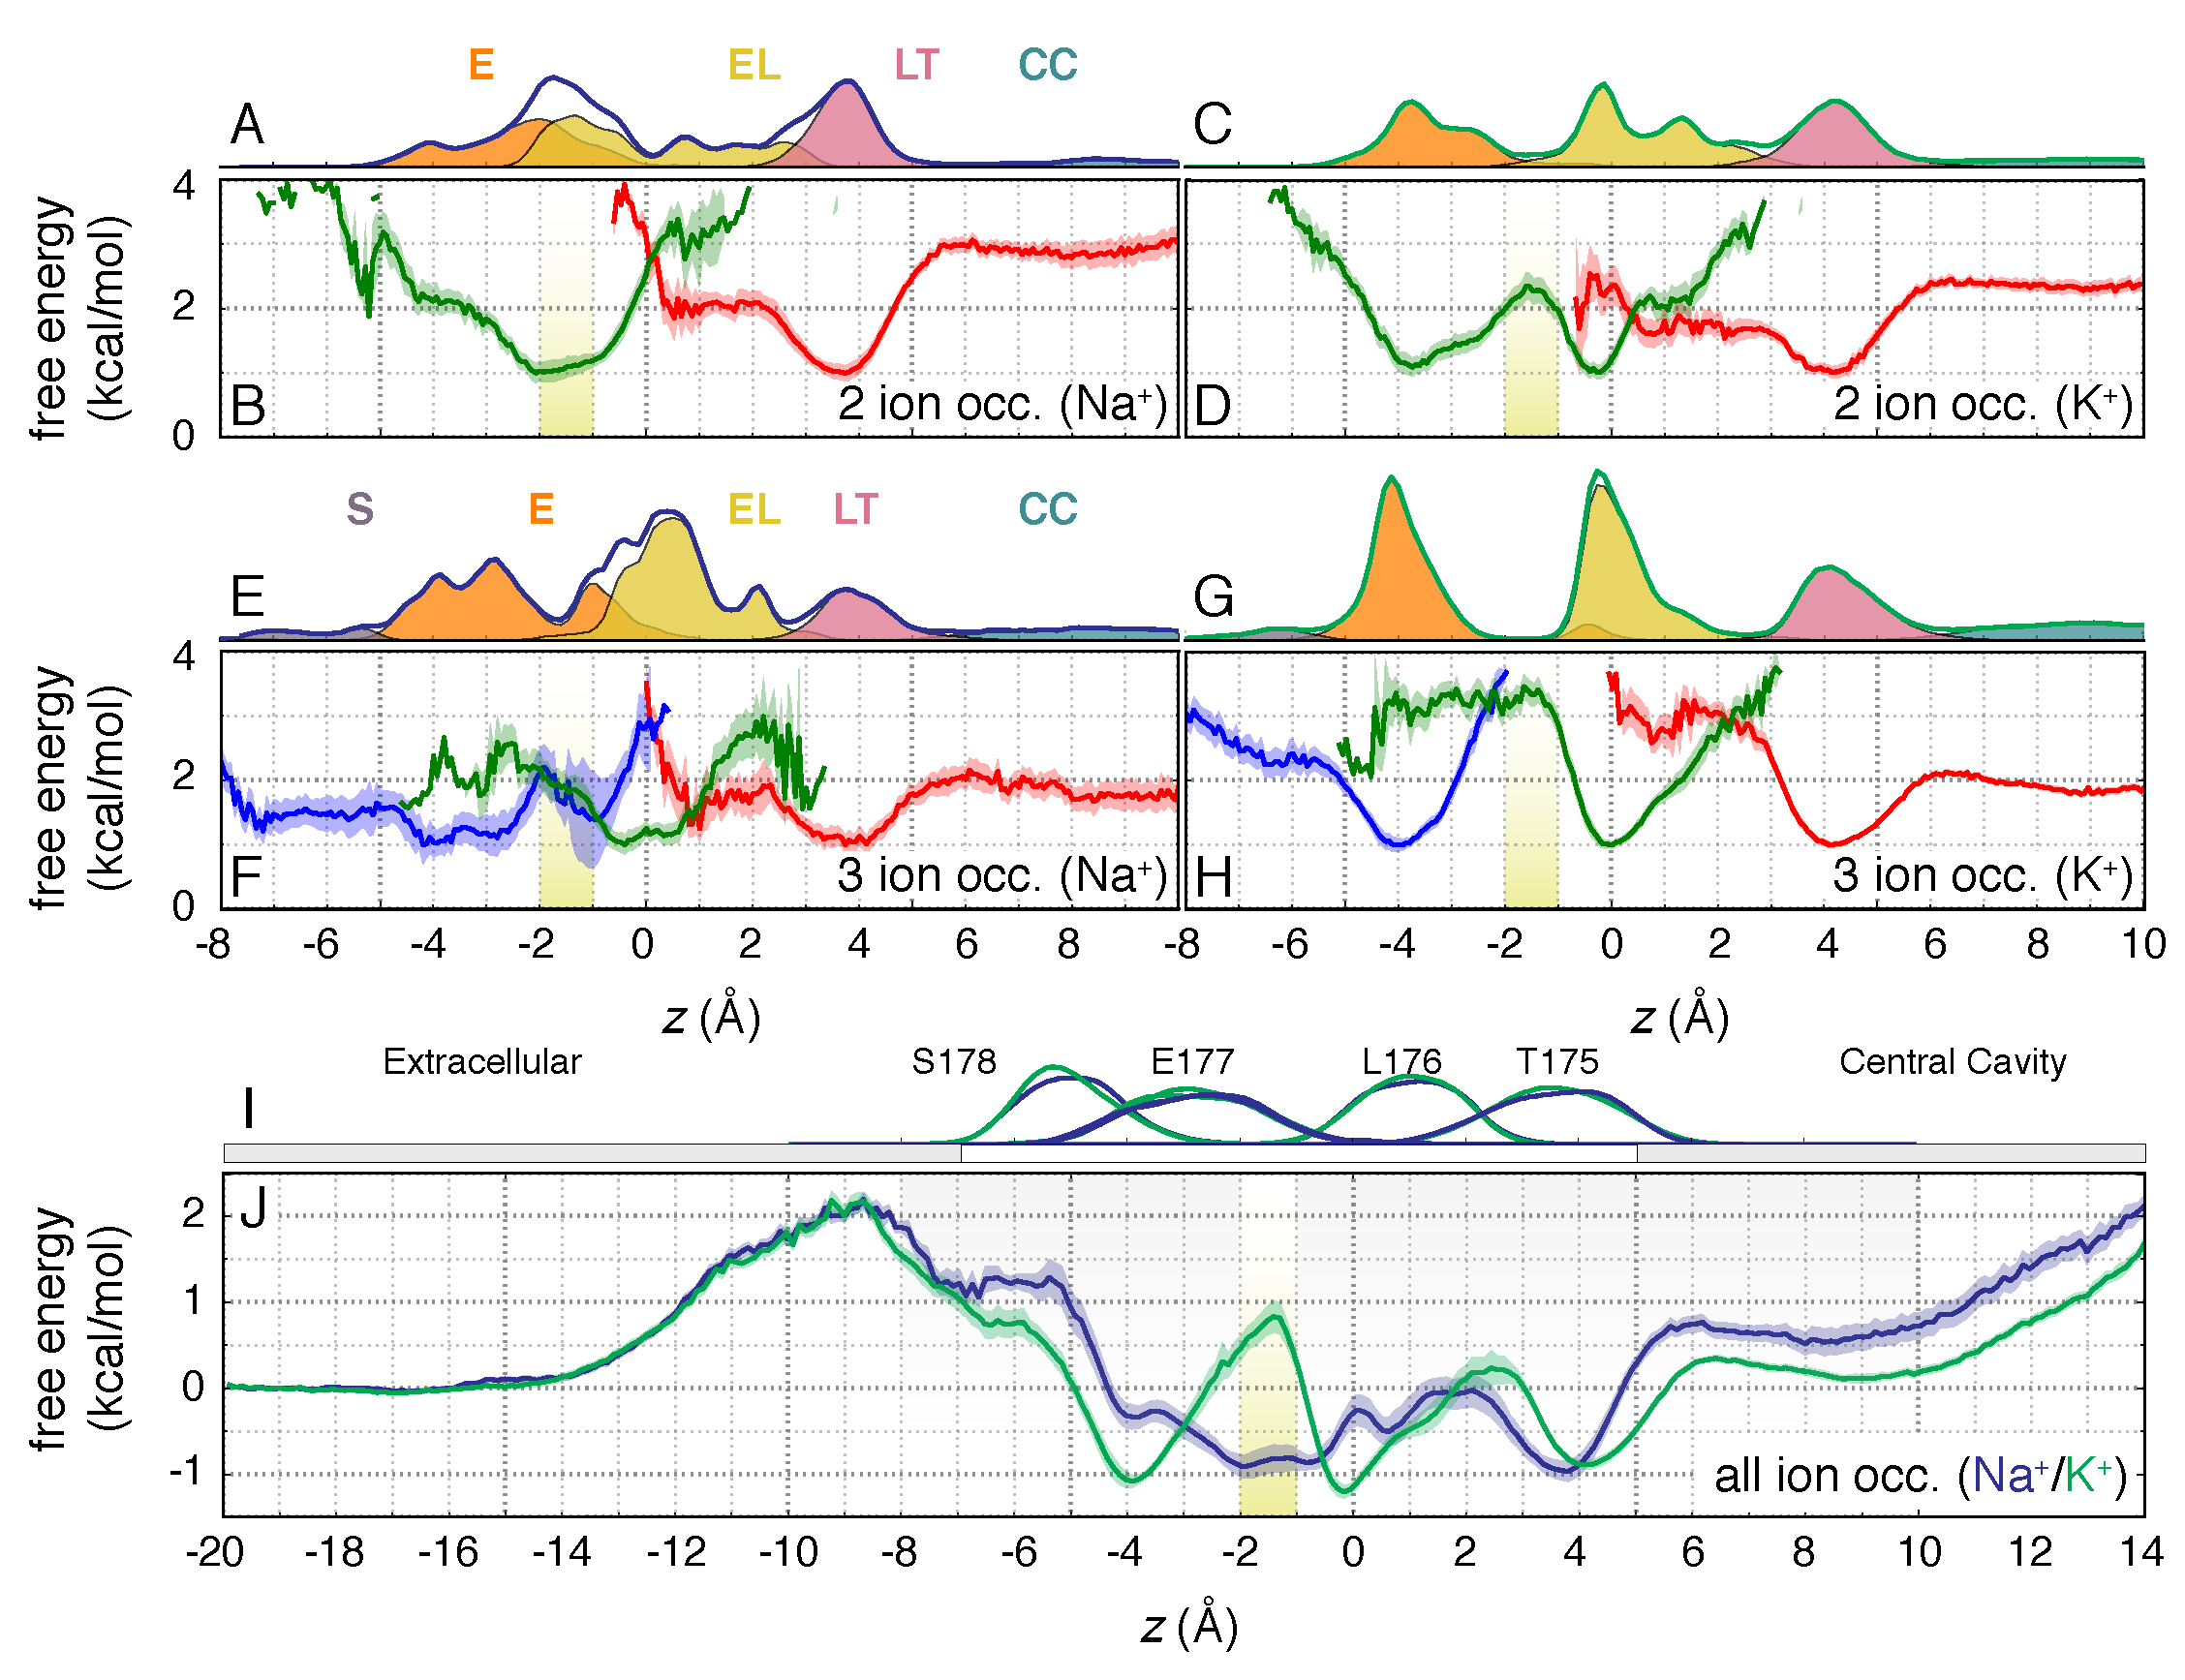
\includegraphics[width=0.6\textwidth]{nav2/Nav2Fig3-5}
\caption[One-dimensional projection of the multi-ion potential of mean-force (PMF) for the movement of Na$^+$ and K$^+$ along the channel axis in distinct occupancy states]{\textbf{One-dimensional projection of the multi-ion potential of mean-force (PMF) for the movement of Na$^+$ and K$^+$ along the channel axis in distinct occupancy states}. (\textbf{A, C}) Distribution of Na$^+$ or K$^+$ along the pore axis for two ion occupancy of the SF, with colored sub-distributions representing the coordination groups of a permeating ion at that axial position. One-dimensional PMFs for (\textbf{B}) Na$^+$ and (\textbf{D}) K$^+$ movement along the channel axis. Ions are ranked by axial position from CC to EC with the colors `red', and `green' for both ion types. (\textbf{E, G}) Distribution of Na$^+$ or K$^+$ along the pore axis for three ion occupancy of the SF with identical coloring to panels (A, C). One-dimensional PMFs for (\textbf{F}) Na$^+$ and (\textbf{G}) K$^+$ movement along the channel axis. Ions are ranked by axial position from CC to EC with the colors `red', `green', and `blue' for both ion types. (\textbf{I}) Axial distribution of channel oxygen atoms, for both Na$^+$ (blue) and K$^+$ (green) simulations. (\textbf{J}) One-dimensional multi-ion PMFs for ionic movement of Na$^+$ (blue) and K$^+$ (green) extended into the extracellular bulk region (set as the free-energy reference state).}
\label{fig:nav2fig3-5}
\end{figure}

The free-energy barrier for K$^+$ conduction in the 2 ion occupancy state, identified in the 2D PMF surfaces (Fig. \ref{fig:nav2fig3} B,D,F), is qualitatively visible in the 1D projection of the free-energy profile using the positions of all Na$^+$ or K$^+$ cations, respectively (Fig. \ref{fig:nav2fig3-5} J). Na$^+$ moves relatively unimpeded (<1 kcal/mol barriers) through the SF whereas a $\sim$1.5-2 kcal/mol barrier separates the `E' and `EL' binding sites for K$^+$ (identified throughout the manuscript with a gold shaded region, Fig. \ref{fig:nav2fig3-5} J). Note that these pseudo-PMFs obscure the true height of the free energy barriers due to the overlap of both two and three ion states, as well as the multi-ion occupancy of certain free energy basins, but can be used as a short-hand signature of the actual free energy landscape. 

2D PMFs indicate that the ionic occupancy modifies the free energy surface for the innermost red ion, promoting ion translocation into the `CC' the 3 ion state. However, we do not make the assumption that an ion in the central cavity is a valid description of the fully translocated ion (see Discussion), but focus on the entry and exit of ions in and out of the SF. The fluxes between the 2 and 3 occupancy states are computed for Na$^+$ and K$^+$ in both the PD+VSD and PD models (Fig. \ref{fig:nav2figS8}). The forward and backward flux between these occupancy macrostates are roughly equivalent, suggesting that ion rearrangement within the SF are near equilibrium on the timescale of our simulations. In pure cation simulations, K$^+$ exchanges between 2 and 3 ion states twice as fast as Na$^+$, but this exchange is on the same order of magnitude in mixed cation simulations.

\begin{figure}[!htb]
\centering
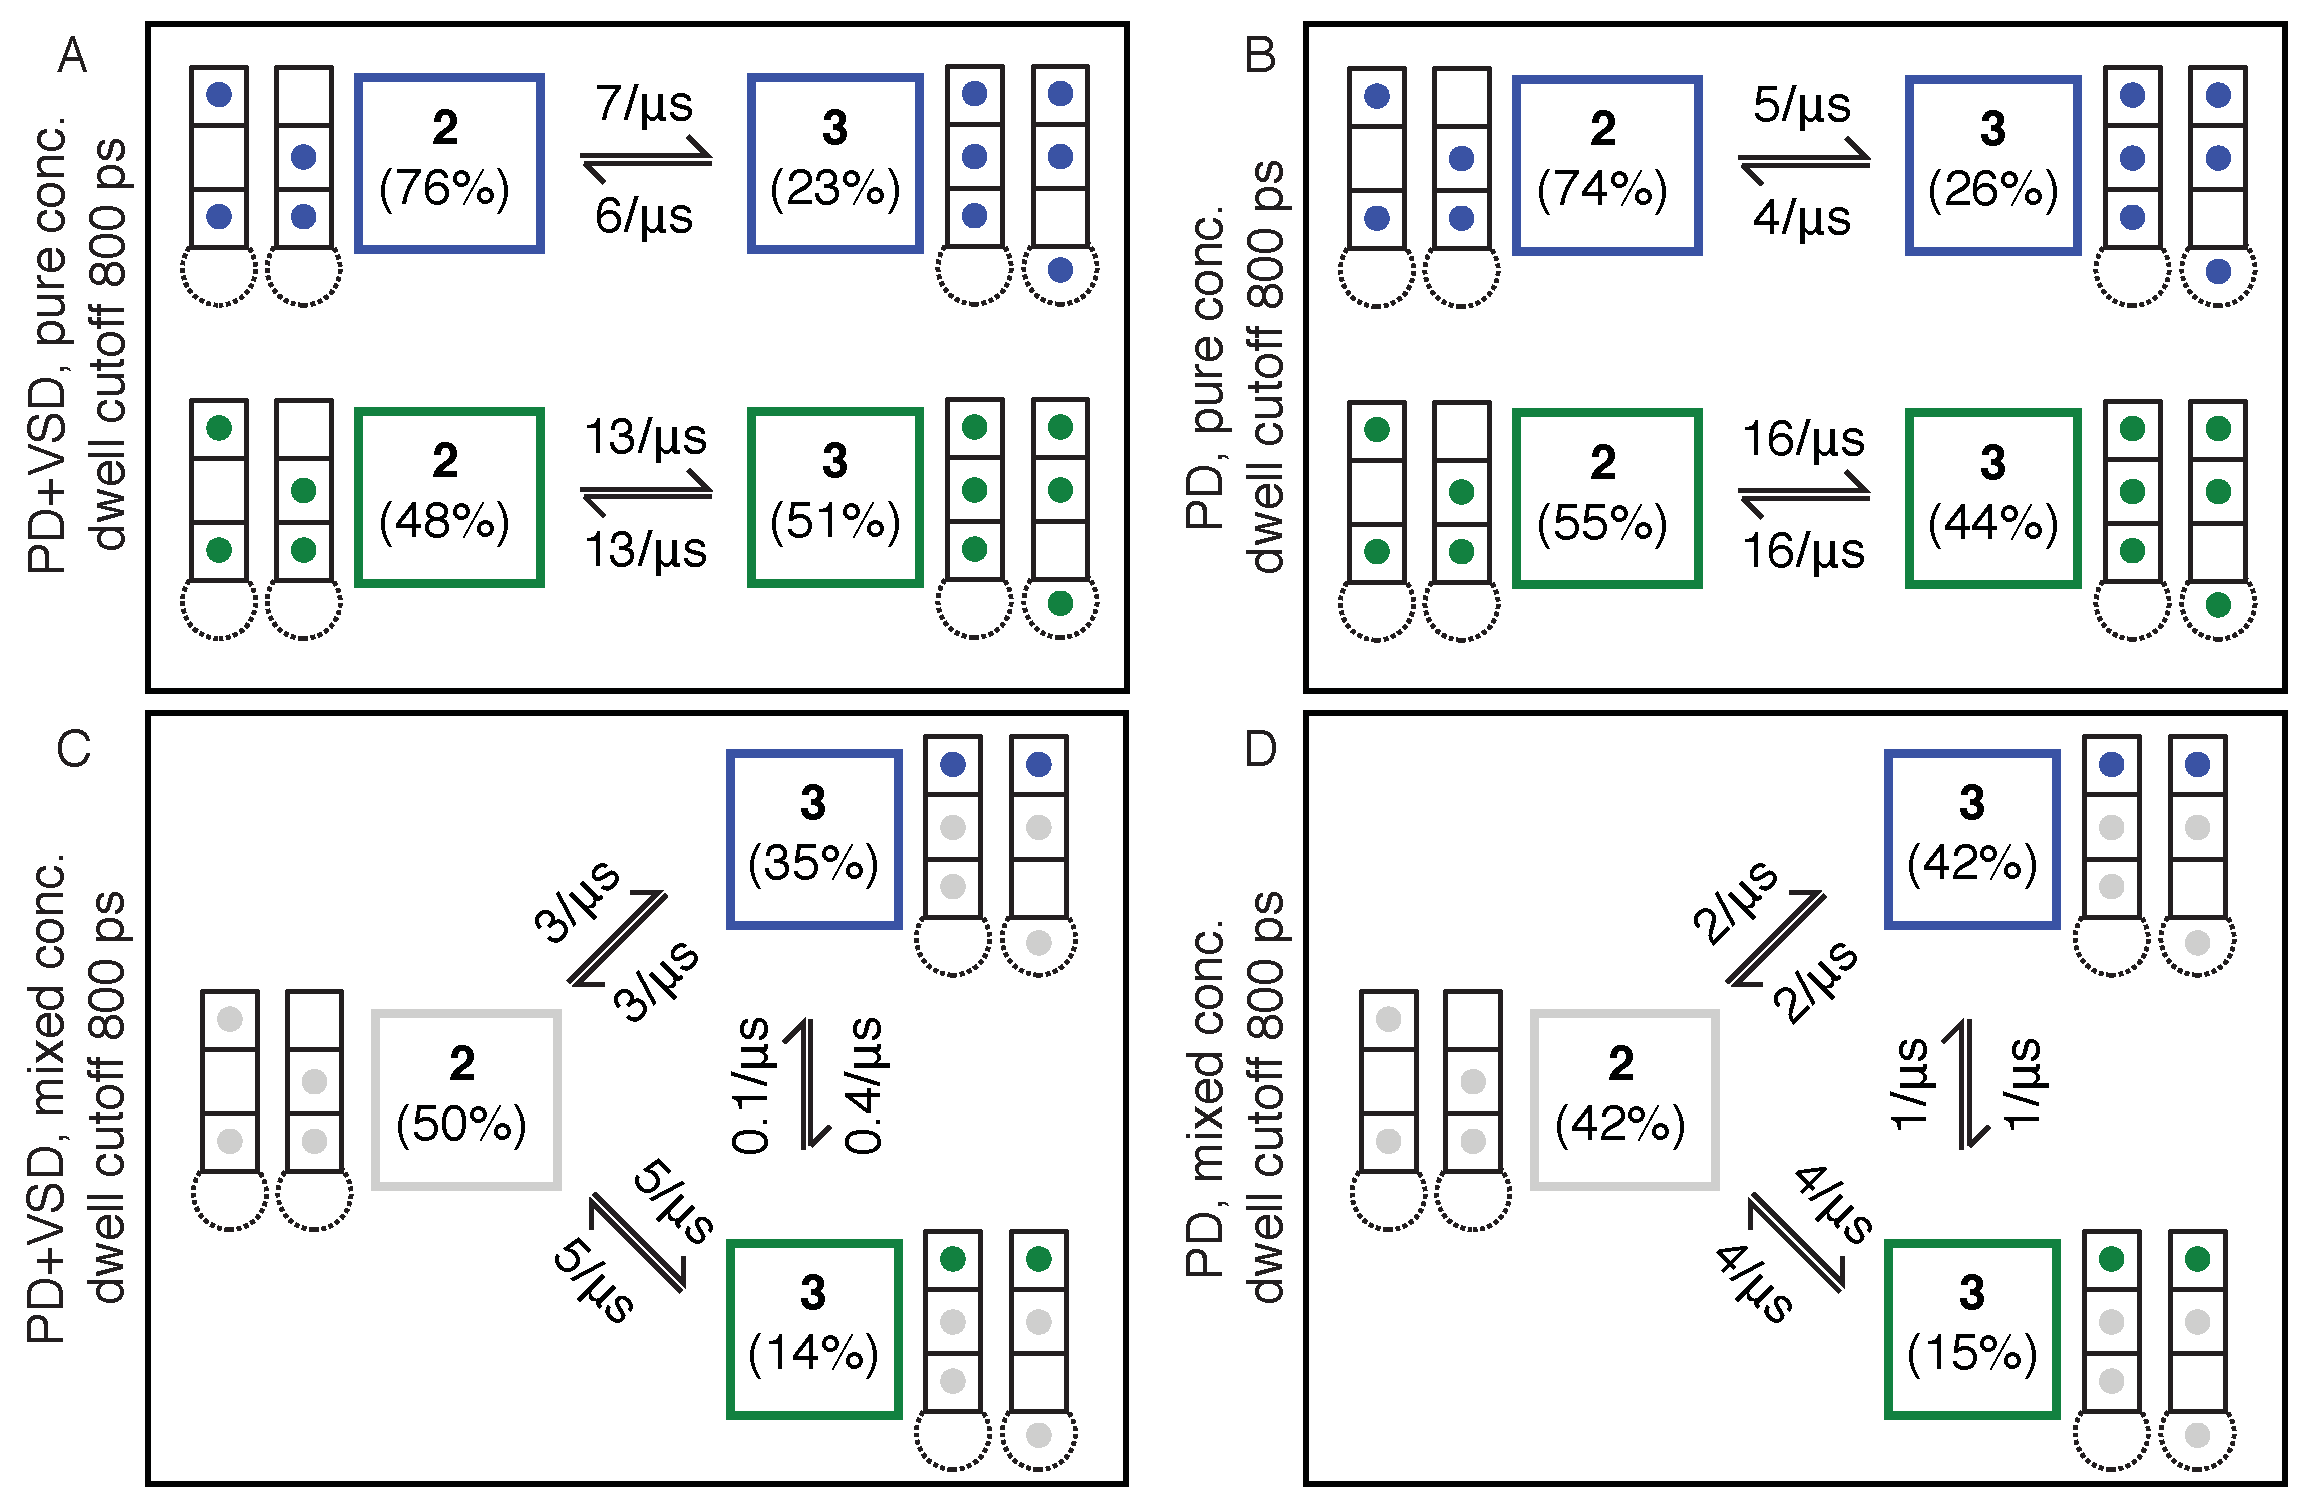
\includegraphics[width=0.6\textwidth]{nav2/Nav2FigS8}
\caption[Occupancy Macrostate Kinetics of Na$^+$ and K$^+$]{\textbf{Occupancy Macrostate Kinetics of Na$^+$ and K$^+$}. Square boxes (blue for Na$^+$, green for K$^+$) represent the primary channel macrostates, 2 and 3, with macrostate populations are shown within each box. Bidirectional arrows between macrostates indicate the average ionic flux between two states across all replicas. Kinetic diagram illustrating ion flux into the SF for pure cation concentrations in the (\textbf{A}) PD+VSD and (\textbf{B}) PD models and ion flux into the SF from mixed cation simulations in the (\textbf{C}) PD+VSD and (\textbf{D}) PD models. In mixed cation simulations, we distinguish between entry of Na$^+$ and K$^+$ to form the 3 ion occupancy state. Transitions between states failing to start and end in a macrostate for a dwell time of 800 ps are removed from this analysis, reducing over-counting of fast transitions.}
\label{fig:nav2figS8}
\end{figure}

\subsection{Mixed Cations in the Na\textsubscript{V}Ab Pore}

\begin{figure}[!htb]
\centering
\includegraphics[width=0.7\textwidth]{nav2/Nav2FigS2}
\caption[Sodium and potassium ion movement in the selectivity filter of Na\textsubscript{V}Ab from a mixed concentration simulations in the PD+VSD model]{\textbf{Sodium and potassium ion movement in the selectivity filter of Na\textsubscript{V}Ab from a mixed concentration simulations in the PD+VSD model}. (\textbf{A}) Representative snapshots of Na$^+$ (blue spheres) and K$^+$ ions (green spheres) in the SF are shown at specified time steps. The pore-lining oxygen groups of the SF (backbone carbonyl groups of T175 and L176 and the side chains of E177 and S178) are shown. (\textbf{B, D}) Dynamics of Na$^+$ and K$^+$ ions along the pore axis from different simulation repeats. Colored bars at the bottom of each time series indicate the channel occupancy (legend in top right). Distribution of (\textbf{C}) Na$^+$ or (\textbf{E}) K$^+$ cations along the pore axis over all simulation repeats, with colored sub-distributions indicating which of the SF residues T, L, E, S coordinate a permeating ion at that axial position. Distributions are normalized by channel average channel occupancy of each ion type. }
\label{fig:nav2figS2}
\end{figure}

%In addition, electrophysiological measurements of Na\textsubscript{V}Ab were performed successively in pure cation and bi-ionic conditions (Fig. \ref{fig:nav2figS11}). Relative permeabilities computed using either the ratio of normalized peak conductance or the reversal potential confirm that Na\textsubscript{V}Ab is permeable to cations in mixed cation concentrations, in agreement with the measured selectivity of bacterial channel NaChBac \cite{FinolUrdaneta:2014bz}.

We studied competitive binding of Na$^+$ and K$^+$ in the SF using MD simulations in presence of mixed NaCl and KCl solutions. Four selected time trajectories of mixed NaCl and KCl solutions in the PD+VSD model reveal a diverse number of ionic arrangements within the SF (Fig.  \ref{fig:nav2figS2}). Na$^+$ and K$^+$ may occupy the same axial position in the `EL' binding site, permitting exchanges of these ions within the SF (Fig. \ref{fig:nav2figS2} A iv, v). Average axial distributions of Na$^+$ and K$^+$ across all simulation repeats show that all the binding sites found in pure cation simulations are occupied (Fig. \ref{fig:nav2figS2} C,E). A projected free energy barrier separating the `E' and `EL' sites is still seen in the multi-ion PMF for K$^+$ in mixed cation simulations (Fig. \ref{fig:nav2fig4} C). Although the relative binding affinities of the `E', `EL', and `LT' sites are unchanged for Na$^+$ and K$^+$ (Fig. \ref{fig:nav2fig4} C), there is a difference in occupancy of these sites. Overall, ion occupancy of the pore is mixed 66\% of the time, whereas Na$^+$-only and K$^+$-only occupancy are observed 34 and 0\% of the time, respectively (see the most populated channel configurations in Fig. \ref{fig:nav2fig4} H). Cation competition has dramatic effects on relative binding propensities in the SF. In pure-cation simulations, the SF is occupied by $2.0 \pm 0.1$ cations for both Na$^+$ and K$^+$ (Fig. \ref{fig:nav2fig2} B), but the SF becomes 25\% more Na$^+$ selective when the two cations are competing ($1.21 \pm 0.04$ vs. $0.97 \pm 0.04$, for Na$^+$ and K$^+$, respectively, Fig. \ref{fig:nav2fig4} G). Binding occupancies of the competing ions show 86\% and 20\% preferences for Na$^+$ over K$^+$ in the `E' and `EL' sites, respectively, corresponding to a free energy difference of $\sim 0.5$kT at 300 K. Even though Na$^+$ and K$^+$ do not share a binding site in the highest population ionic configurations within the channel (Fig. \ref{fig:nav2fig4} H), all-ion pair 2D PMFs show that it is possible for Na$^+$ to pass itself and K$^+$ in mixed cation simulations (Fig. \ref{fig:nav2figS7} C-E).

\begin{figure}[!ptb]
\centering
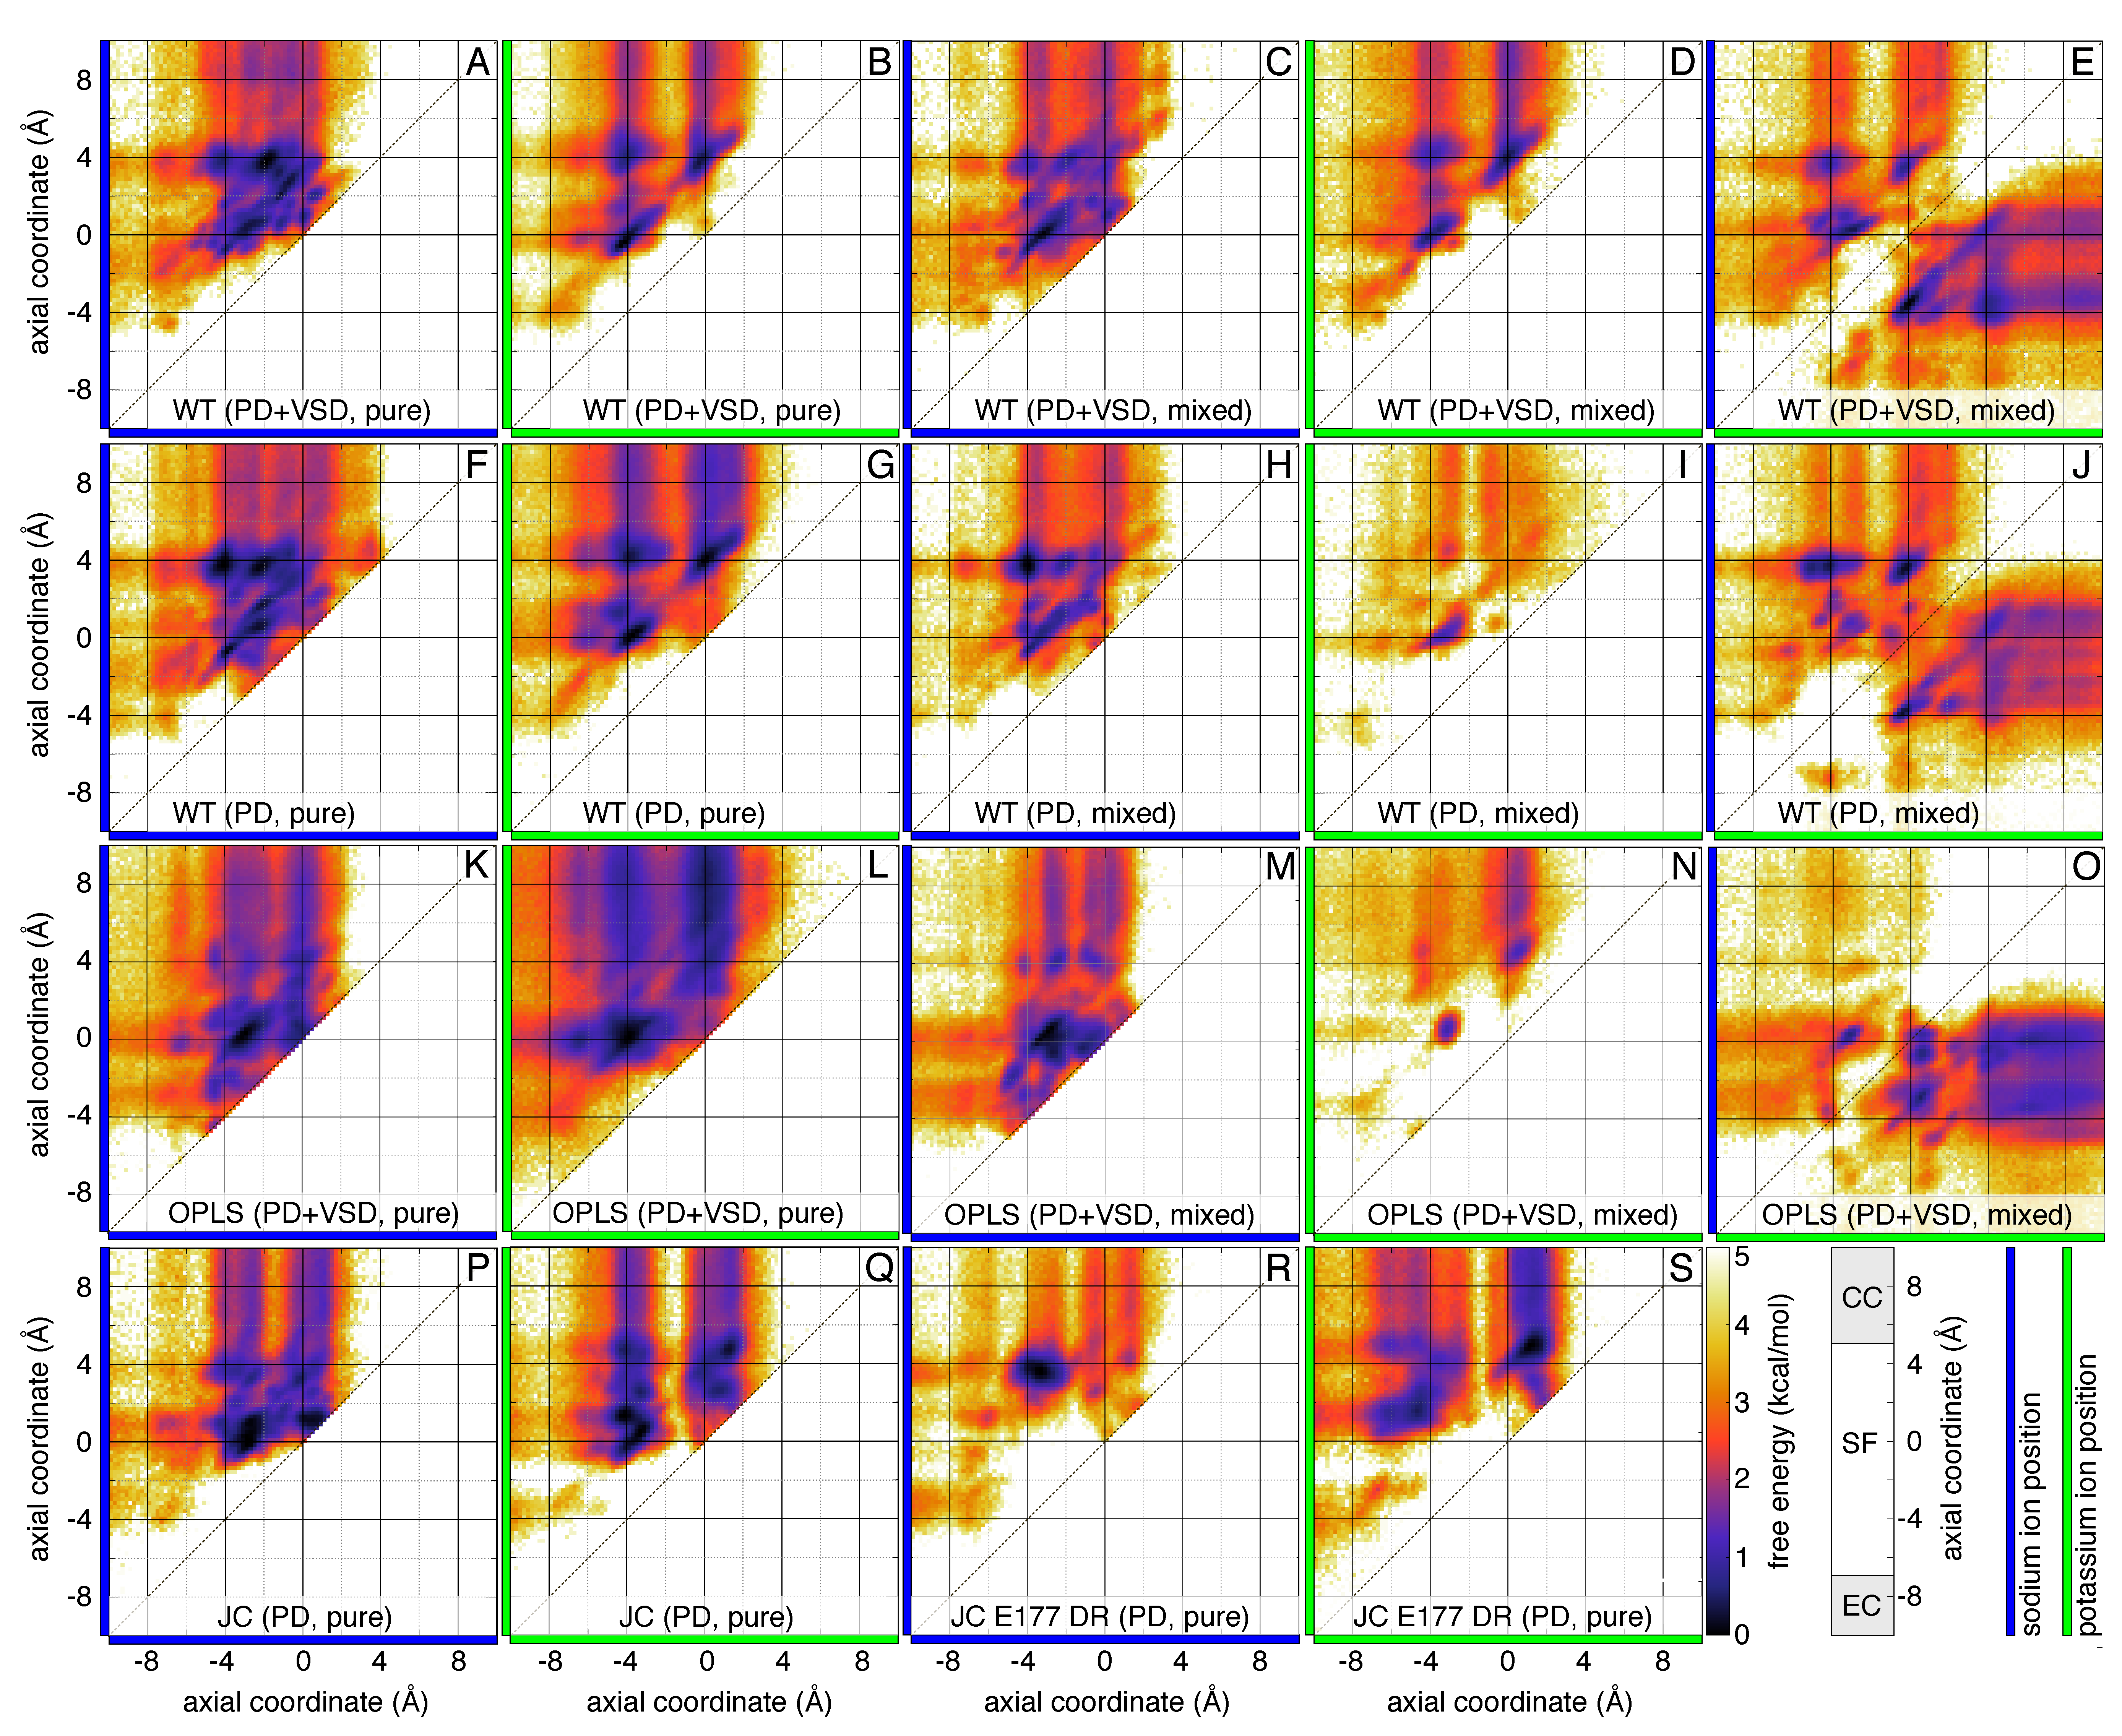
\includegraphics[width=0.7\textwidth]{nav2/Nav2FigS7}
\caption[Two-dimensional potential of mean-force (PMF) for Na$^+$ and K$^+$ pairs along the channel axis]{\textbf{Two-dimensional potential of mean-force (PMF) for Na$^+$ and K$^+$ pairs along the channel axis}. Ionic species are identified by a colored bar on the axes, Na$^+$ (blue) and K$^+$ (green). PMFs for (\textbf{A}) Na$^+$-Na$^+$ and (\textbf{B}) K$^+$-K$^+$ in pure cation simulations, and (\textbf{C-E}) Na$^+$-Na$^+$, K$^+$-K$^+$, and Na$^+$-K$^+$ in mixed cation simulations in the PD+VSD model. (\textbf{F}) Na$^+$-Na$^+$ and (\textbf{G}) K$^+$-K$^+$ in pure cation simulations, and (\textbf{H-J}) Na$^+$-Na$^+$, K$^+$-K$^+$, and Na$^+$-K$^+$ in mixed cation simulations in the PD model. PMFs for the (\textbf{K-O}) OPLS model, (\textbf{P-Q}) JC model, and (\textbf{R-S}) JC model E177 dihedral restraints. The reference state (zero free energy) is set to the high probability state for each pure cation or mixed cation simulation dataset, respectively.}
\label{fig:nav2figS7}
\end{figure}

\begin{figure}[!htb]
\centering
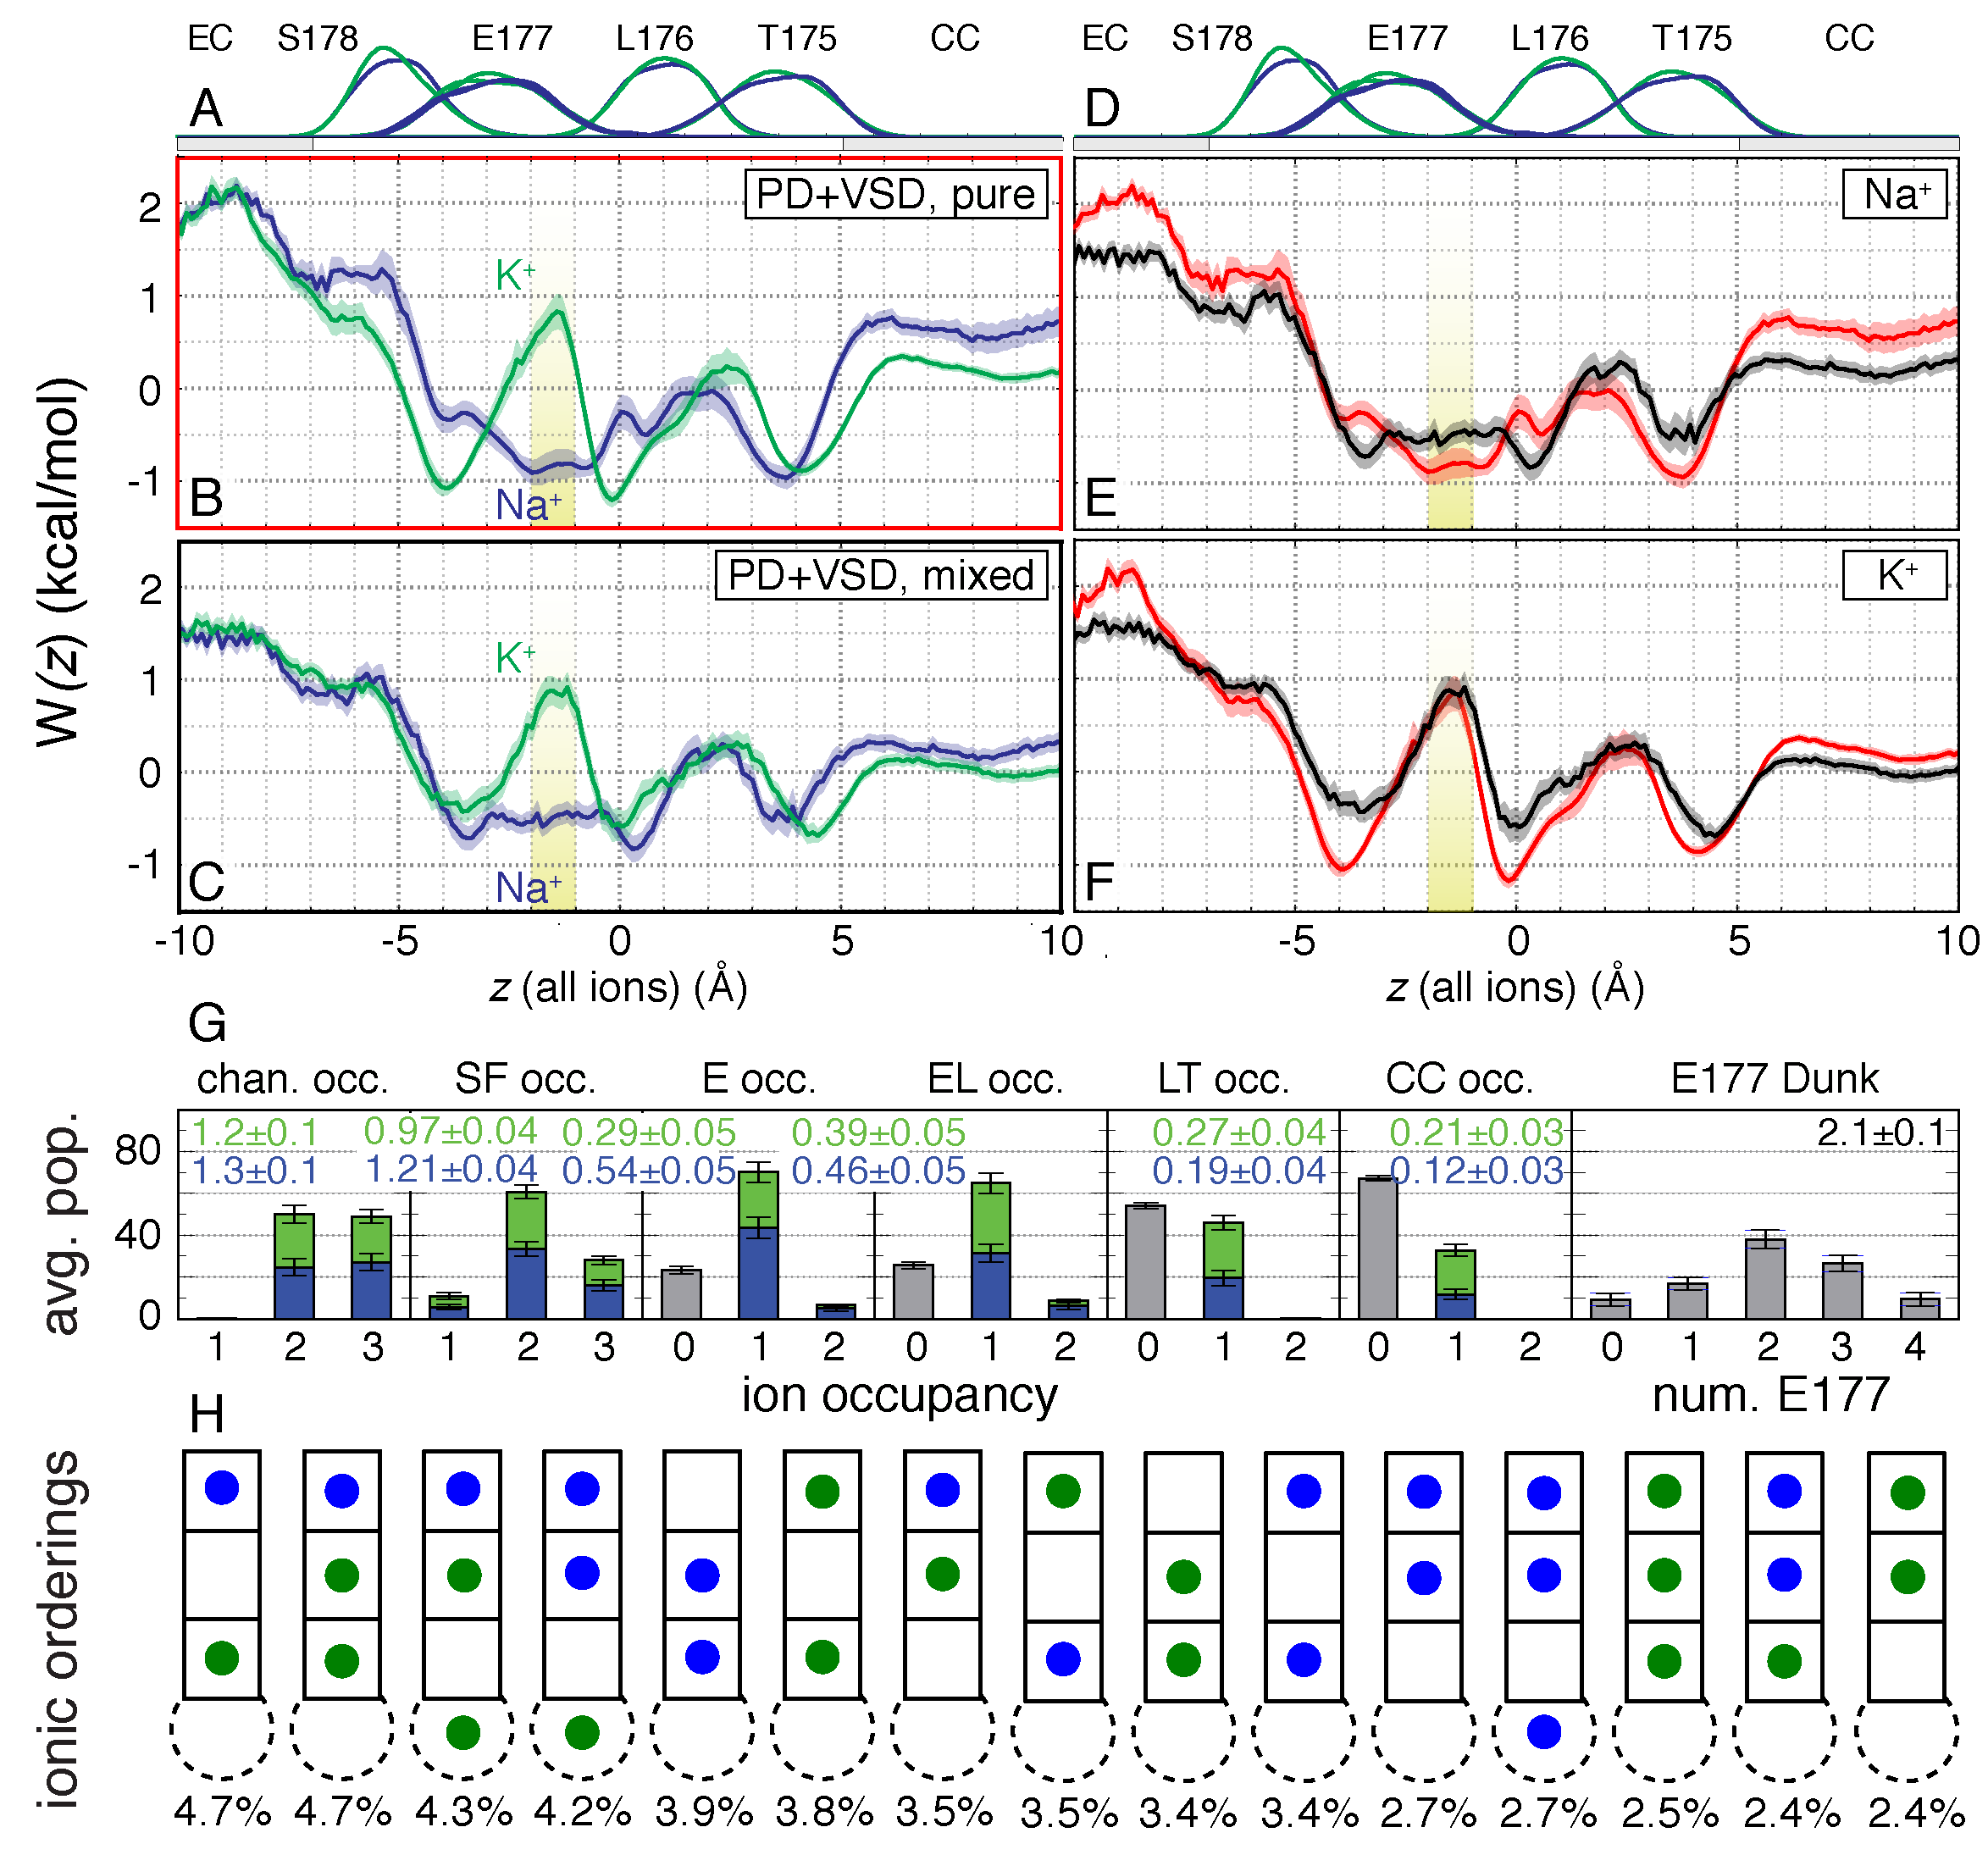
\includegraphics[width=0.6\textwidth]{nav2/Nav2Fig4}
\caption[The effect of competitive binding of Na$^+$ and K$^+$ along the channel axis]{\textbf{The effect of competitive binding of Na$^+$ and K$^+$ along the channel axis}. (\textbf{A,D}) Axial distribution of channel oxygen atoms. One-dimensional multi-ion PMFs for ionic movement of (\textbf{B}) pure Na$^+$ (blue) and K$^+$ (green) and (\textbf{C}) mixed Na$^+$ and K$^+$ along the channel axis in the PD+VSD model. To help comparison between datasets, an overlays of 1D multi-ion PMFs for (\textbf{E}) Na$^+$ and (\textbf{F}) K$^+$ are also shown. The reference state (zero free energy) is defined as the bulk extracellular value of Na$^+$ and K$^+$ separately. A gold band indicates the region of highest free-energy barrier for K$^+$ permeation within the SF. The axial distribution of pore-lining oxygen atoms of T175, L176, E177, and S178 are shown from PD+VSD simulations for Na$^+$ (blue) and K$^+$ (green) above panels (A, D). Ionic occupancy is shown from left to right for the entire channel, the SF, all major binding sites within the SF, together with the number of dunked E177 side chains for (\textbf{F}) mixed cation simulations. (\textbf{G}) Ionic occupancy of binding sites (E, EL, LT, CC) in the highest population channel configurations from mixed cation simulations.}
\label{fig:nav2fig4}
\end{figure}

\subsection{Solvation of Na$^+$ and K$^+$ During Permeation}

\begin{figure}[!ptb]
\centering
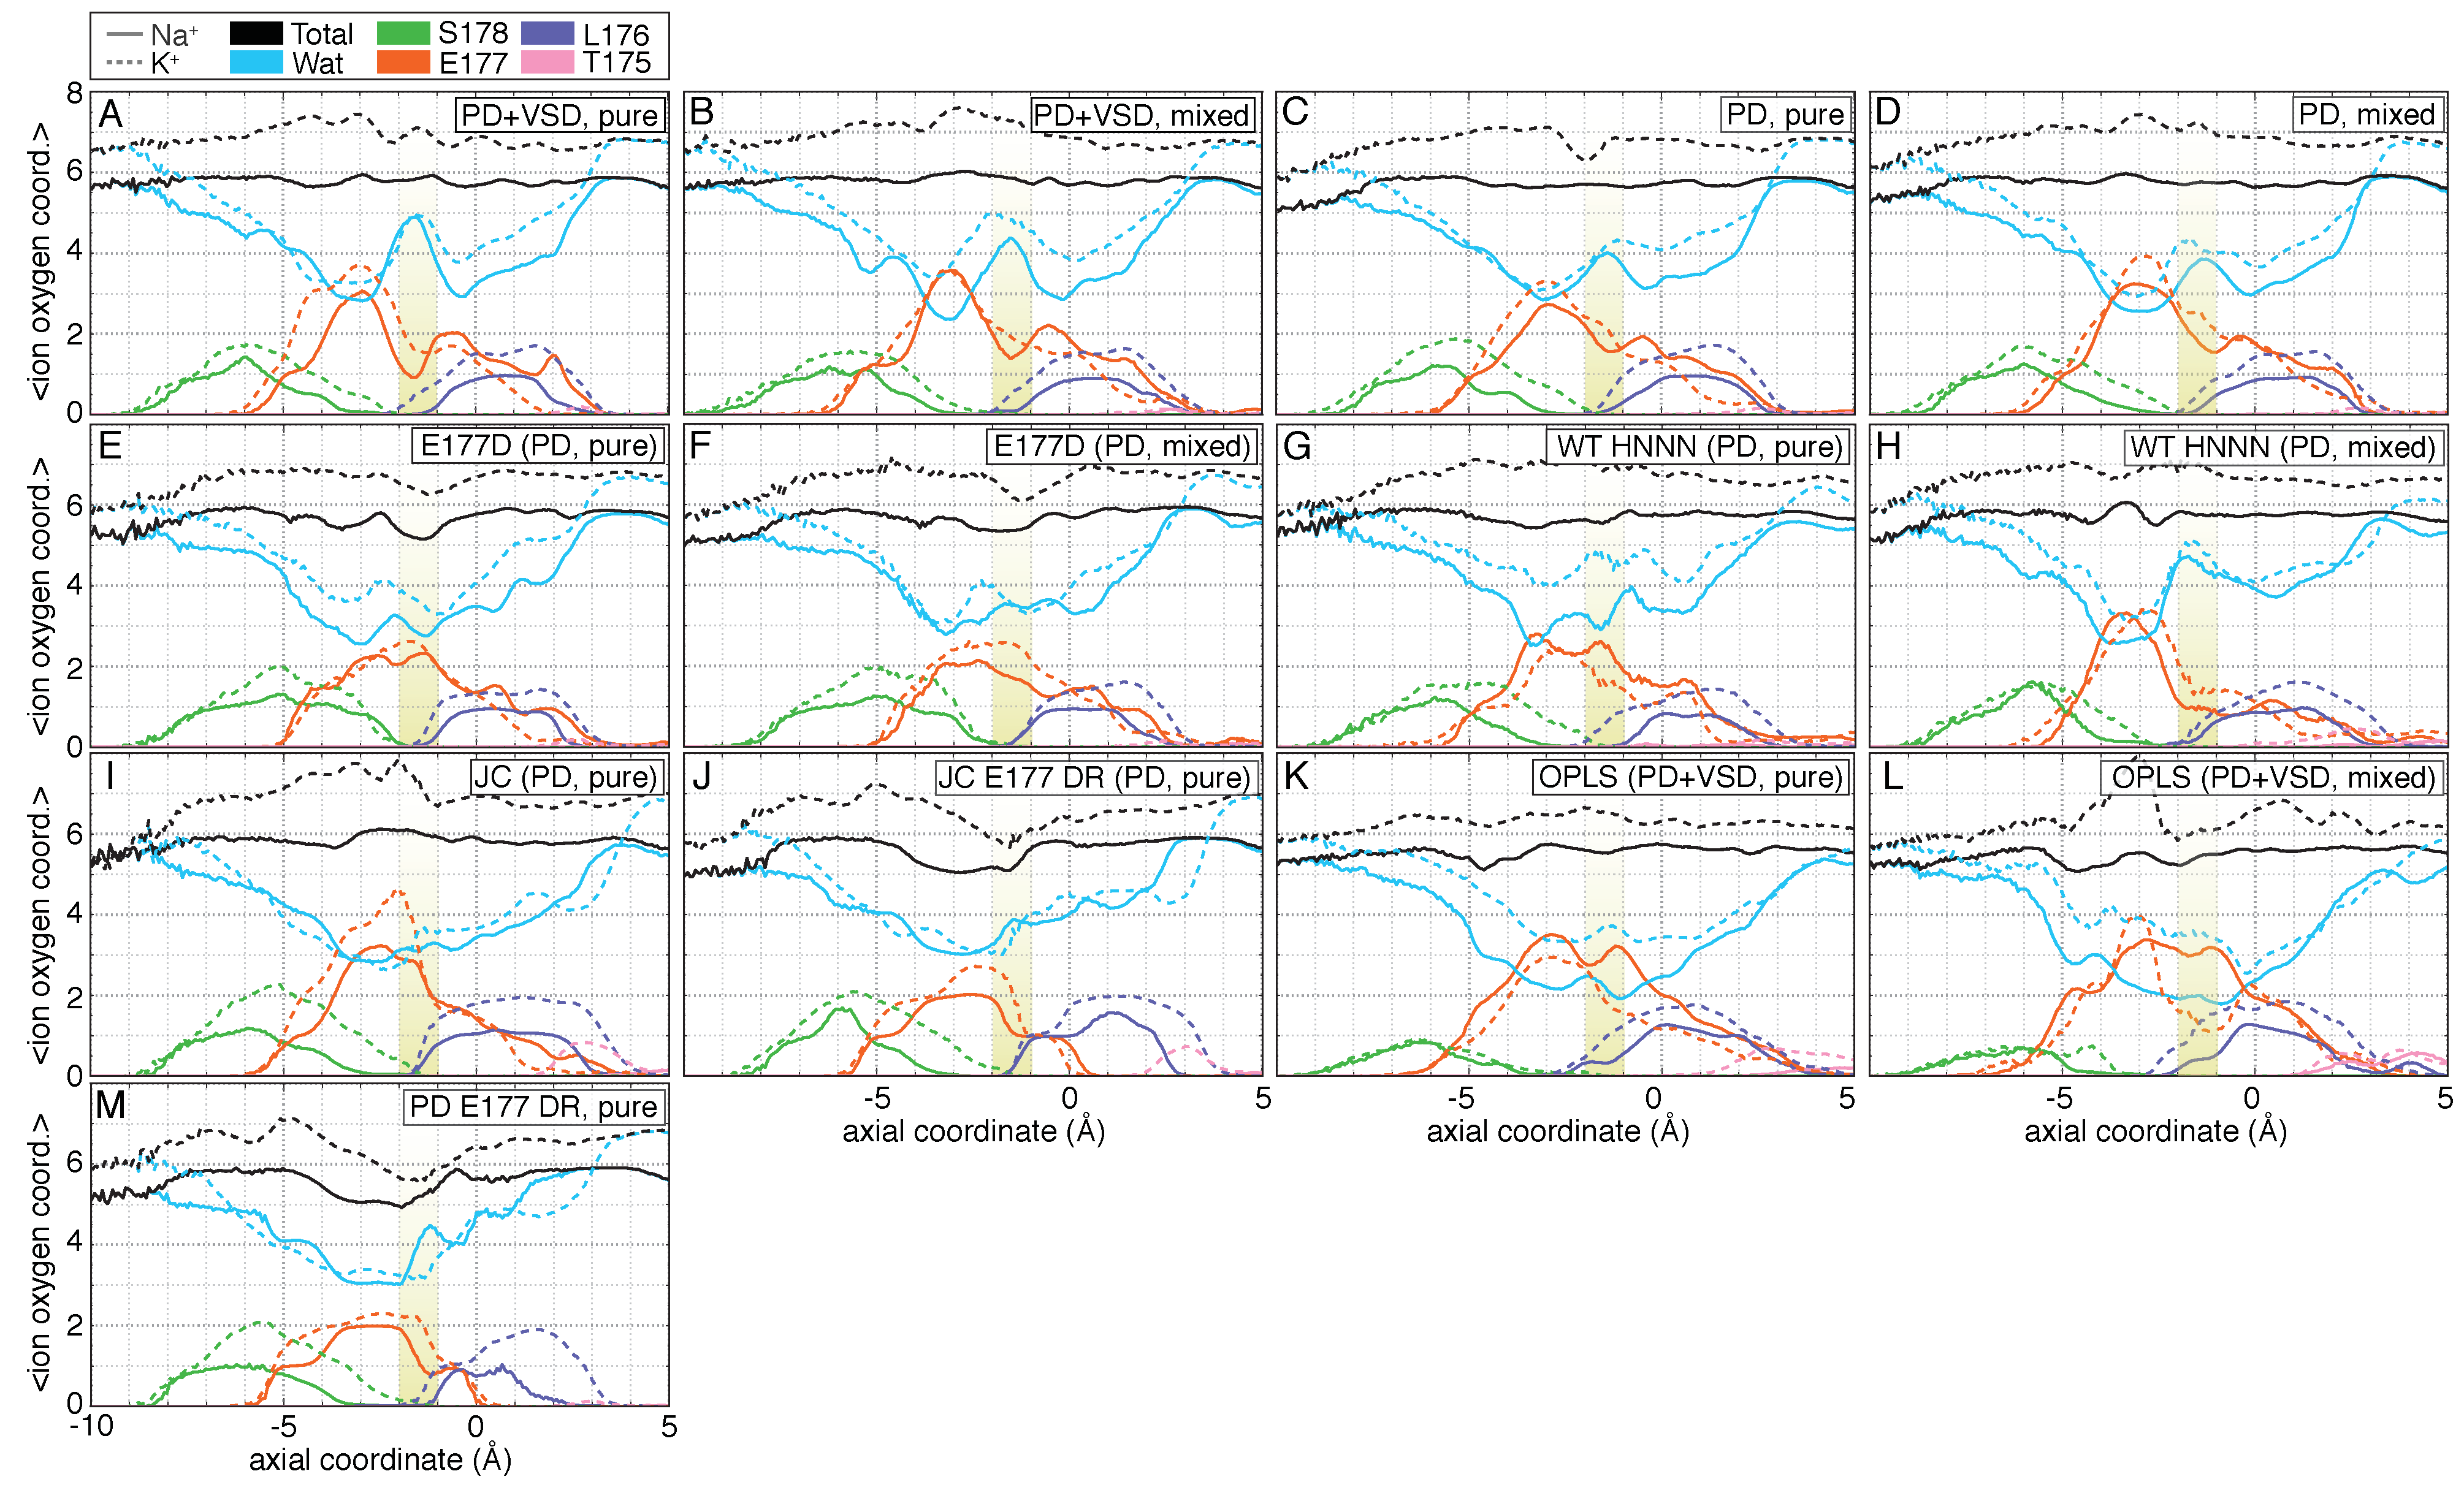
\includegraphics[width=0.9\textwidth]{nav2/Nav2FigS5}
\caption[Average oxygen coordination of Na$^+$ or K$^+$]{\textbf{Average oxygen coordination of Na$^+$ or K$^+$}. The average number of oxygen atoms in the 1st coordination shell of Na$^+$ (solid) and K$^+$ (dashed) as a function of position on the channel axis. Data is shown for the (\textbf{A-B}) PD+VSD model, (\textbf{C-D}) PD model, (\textbf{E-F}) E177D model (where E177 is replaced with D177), (\textbf{G-H}), HNNN model, (\textbf{I-J}) JC model with and without E177 dihedral restraints, the (\textbf{K-L}) OPLS model, and the (\textbf{M}) PD model with E177 dihedral restraints. Individual contributions to the total coordination (black) is depicted for each channel ligand; T175 (pink), L176 (purple), E177 (orange), S178 (green), in addition to water (blue). A gold band indicates the region of highest free-energy barrier for K$^+$ permeation within the SF.}
\label{fig:nav2figS5}
\end{figure}

To examine the basis for preferential binding of Na$^+$ in the SF of Na\textsubscript{V}Ab, we calculate the average coordination of cations by water molecules and channel ligands along the channel axis (Fig. \ref{fig:nav2figS5}).  The average number of O atoms in the first solvation shell varies between 5 and 6 for Na$^+$ and between 6 and 7 for K$^+$, in good quantitative agreement with simulation studies of these two cations in the potassium channel KcsA \cite{Egwolf:2010ki}.  On either side of the SF, the extracellular vestibule or the central cavity, Na$^+$ and K$^+$ are completely hydrated by $5.62\pm0.03$ and $6.51\pm0.02$ water molecules, respectively, and they remain partly hydrated in the SF, where channel coordination is dominated by L176 and E177. Due its larger radius, K$^+$ has marginally higher coordination to channel ligands across the SF than Na$^+$. In the K$^+$ permeation bottleneck, denoted by a gold band, $\sim$1-2 carboxylate O ligands solvate Na$^+$ and K$^+$ together with $\sim$4-5 water molecules, with an additional $\sim$1 carbonyl group for K$^+$ (Fig. \ref{fig:nav2figS5} A). This bottleneck is the position of maximal hydration within the SF for both Na$^+$ and K$^+$ across PD+VSD, PD pure, and PD mixed simulations. Cation solvation is unchanged for Na$^+$ between the pure and mixed cation simulations, but an increase in the number of dunked glutamic acid side chains was observed in mixed cation simulations (Fig. \ref{fig:nav2figS5} A-B). Overall, since solvation is not significantly different for the two cations, and the barrier region corresponds to the maximally hydrated SF position, we conclude that the moderate barrier for K$^+$ at this site is due to the difficulty in hydrating the cation at that location, something which does not occur for Na$^+$. 

\subsection{Effect of conformational isomerization of E177 on cation binding and mobility }

\begin{figure}[!ptb]
\centering
\includegraphics[width=0.7\textwidth]{nav2/Nav2FigS3}
\caption[Sodium and potassium ion movement in the selectivity filter of Na\textsubscript{V}Ab when E177 is restrained in the crystallographic orientation]{\textbf{Sodium and potassium ion movement in the selectivity filter of Na\textsubscript{V}Ab when E177 is restrained in the crystallographic orientation}. (\textbf{A}) Representative snapshots of Na$^+$ (blue spheres) and K$^+$ ions (green spheres) in the SF are shown at specified time steps. The pore-lining oxygen groups of the SF (backbone carbonyl groups of T175 and L176 and the side chains of E177 and S178) are shown. (\textbf{B, D}) Movement of Na$^+$ and K$^+$ ions along the pore axis from different simulation repeats. Colored bars at the bottom of each time series indicate the channel occupancy (legend in top right). (\textbf{C, E}) Distribution of Na$^+$ or K$^+$ along the pore axis over all pure cation simulation repeats, with colored sub-distributions representing the coordination groups of a permeating ion at that axial position. Distributions are normalized by channel average channel occupancy of each ion. (\textbf{F}) Movement of Na$^+$ and K$^+$ ions in a mixed cation simulation with (\textbf{G}) the distribution of Na$^+$ and K$^+$ along the channel axis for all mixed cation simulation repeats.}
\label{fig:nav2figS3}
\end{figure}

\begin{figure}[!htb]
\centering
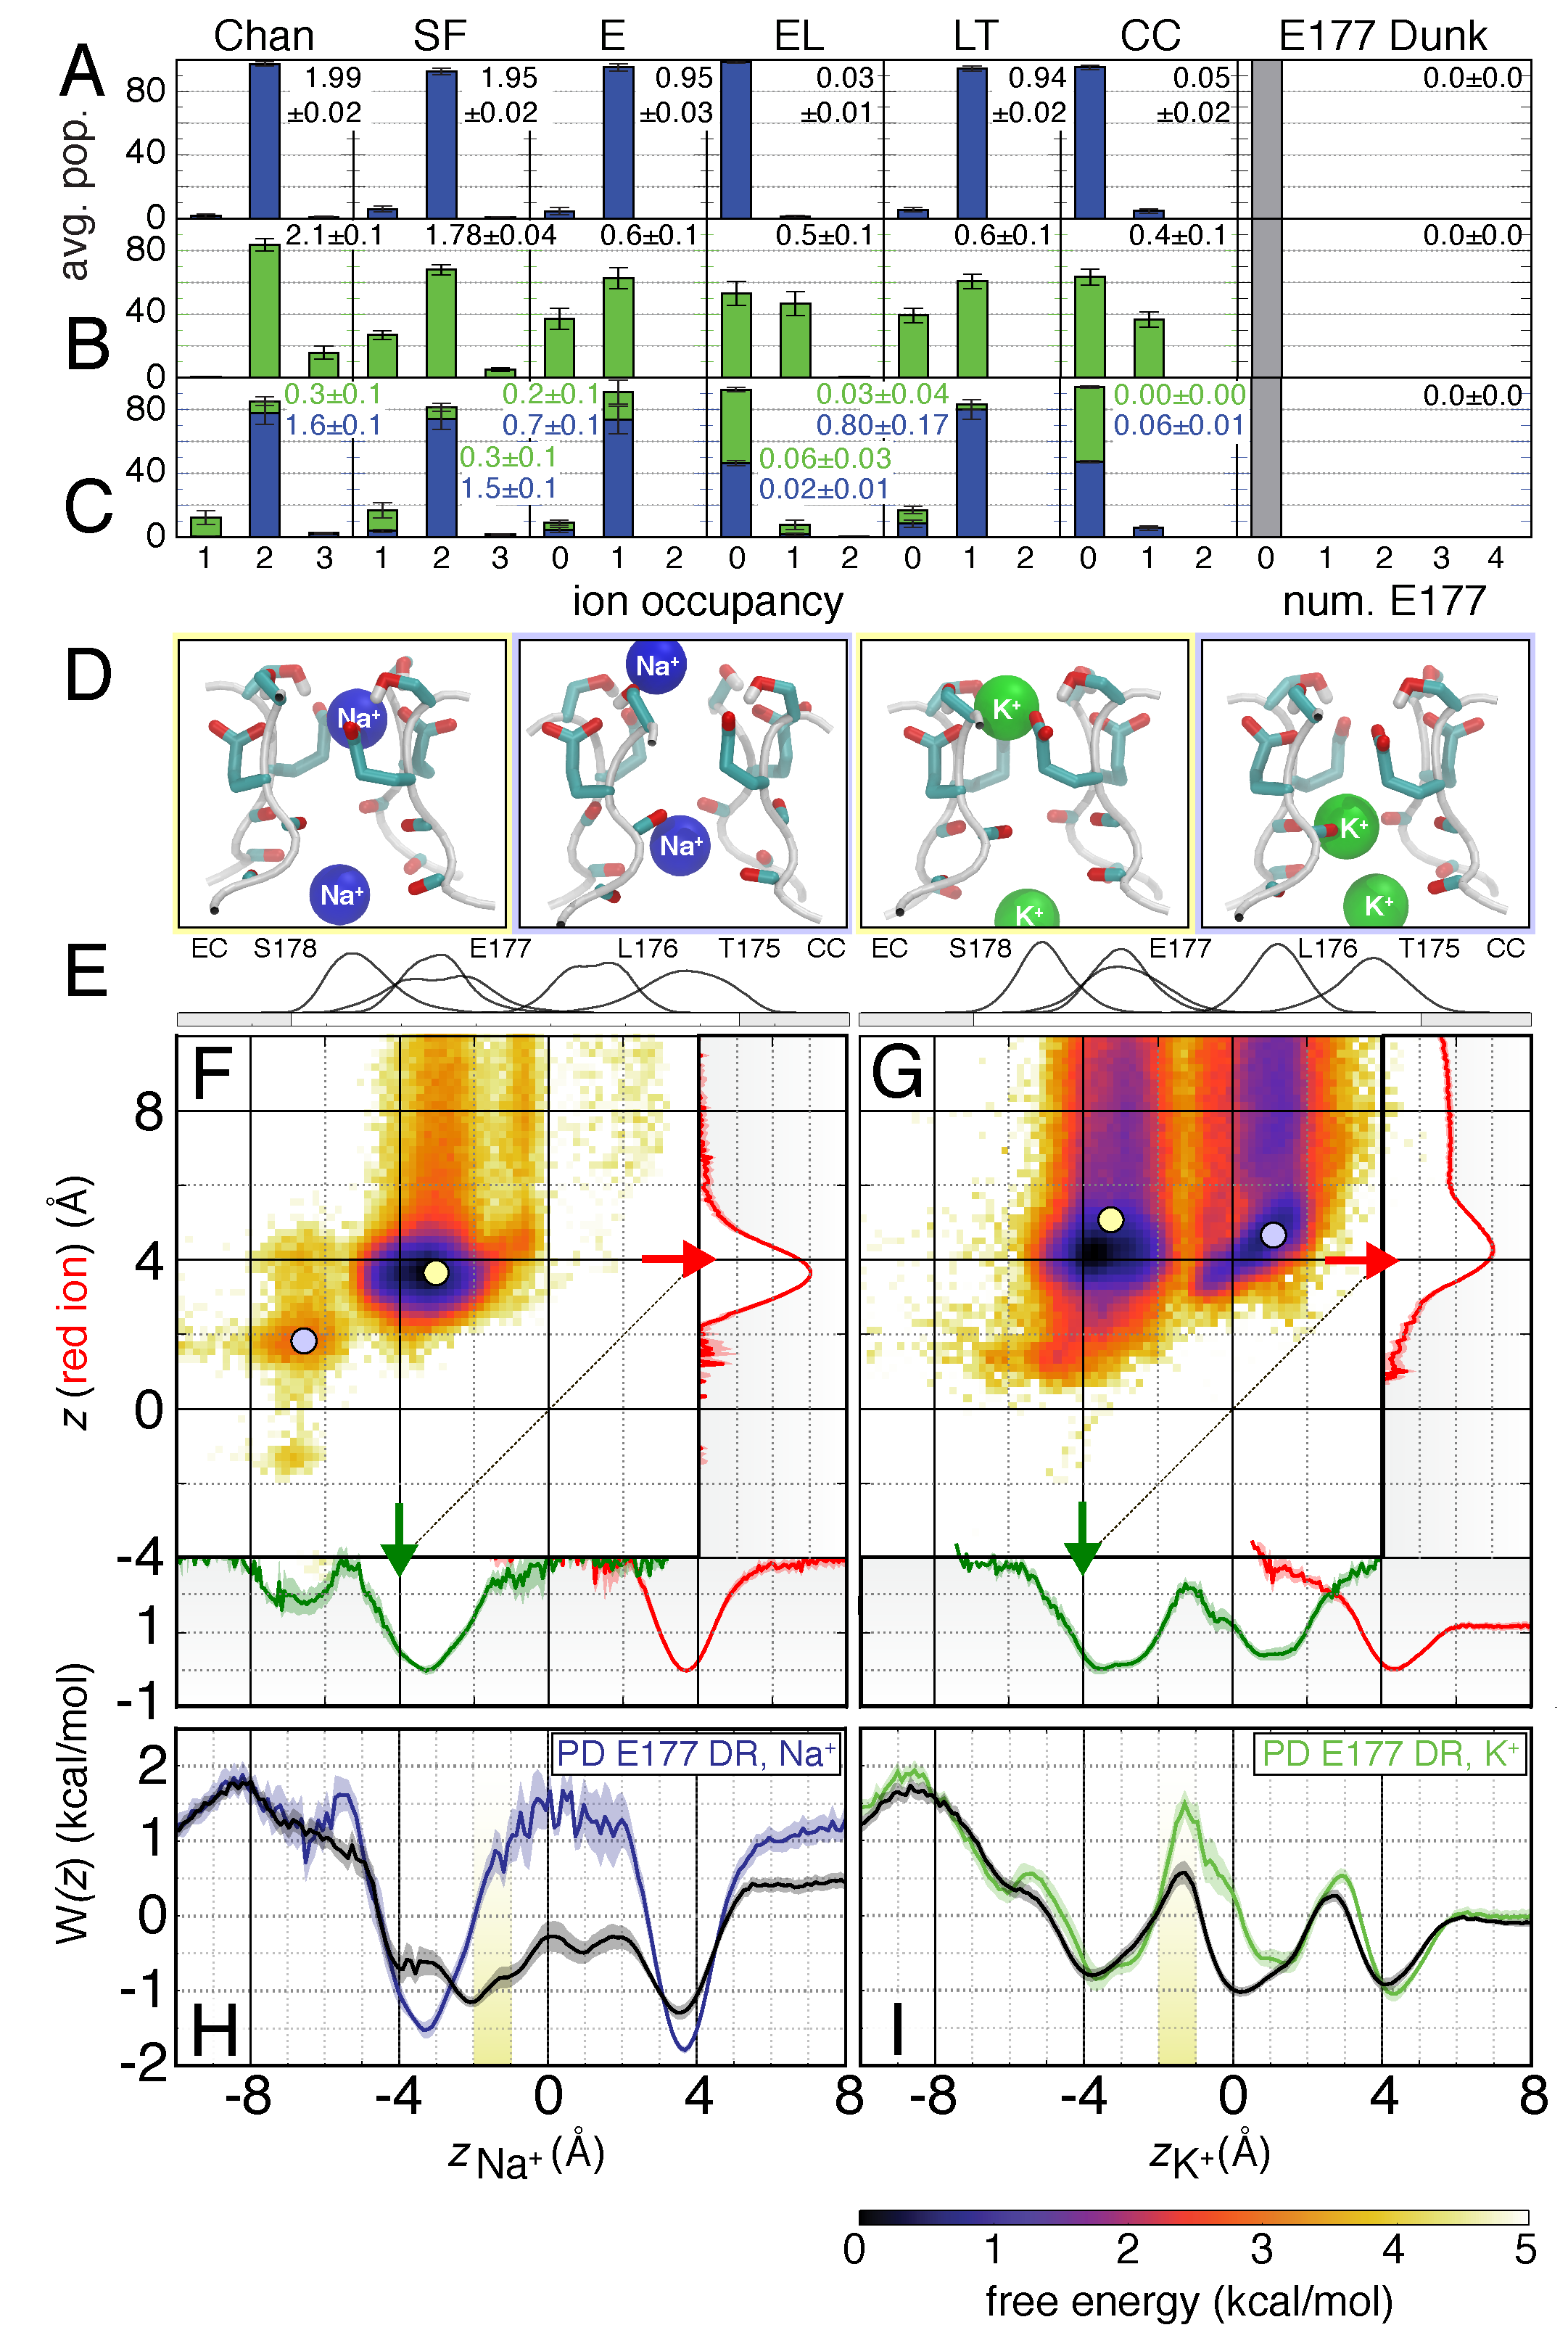
\includegraphics[width=0.6\textwidth]{nav2/Nav2Fig5}
\caption[Binding statistics and potential of mean-force (PMF) for the movement of Na$^+$ and K$^+$ along the channel axis where E177 is restrained in the crystallographic orientation]{\textbf{Binding statistics and potential of mean-force (PMF) for the movement of Na$^+$ and K$^+$ along the channel axis where E177 is restrained in the crystallographic orientation}. (\textbf{A}) Ionic occupancy is shown from left to right for the entire channel, the SF, all major binding sites within the SF, together with the number of dunked E177 side chains, for (\textbf{A}) pure Na$^+$, (\textbf{B}) pure K$^+$, and (\textbf{C}) mixed cation simulations. Values from mixed cation simulations may not reflect equilibrium distributions due to limited ion mobility. (\textbf{D}) Representative snapshots of dominant ion configurations within the SF. (\textbf{E}) The axial distribution of pore-lining oxygen atoms of T175, L176, E177, and S178 for pure Na$^+$ and pure K$^+$ simulations. 2D PMFs for (\textbf{F}) Na$^+$ and (\textbf{G}) K$^+$ are computed between red and green ion pairs for the 2 ion occupancy state. Multi-ion 1D projection onto the channel axis for E177 restrained for (H) Na$^+$ and (I) K$^+$, where a black line in each plot is the 1D PMFs for Na$^+$ and K$^+$ where no restrained were applied, respectively.}
\label{fig:nav2fig5}
\end{figure}

The ionic occupancy of the SF and the probability of E177 dunking are within statistical uncertainty for both simulations with NaCl and KCl (Fig. \ref{fig:nav2fig2} B). As such, it is unclear if E177 conformational isomerization is required for permeation and mediating selectivity. We investigate the influence of E177 side chain conformational fluctuations by restraining them in the crystallographic up-facing orientation (Fig. \ref{fig:nav2fig2} A (right panel)). In E177 restrained simulations, the average channel occupancy is comparable for Na$^+$ and K$^+$, at $2.0\pm0.02$ and $2.1\pm0.1$, respectively. There is a significant drop in occupancy of the 3 ion state for Na$^+$ ($97\pm1$ and $1.6\pm0.4$\% for the 2 and 3 ion states, respectively) and K$^+$ ($84\pm4$ and $16\pm4$\% for the 2 and 3 ion states, respectively) relative to the PD+VSD and PD models without restraints (Fig. \ref{fig:nav2fig5} A,B). For Na$^+$, this decrease in occupancy results from the elimination of binding at the `EL' site (from $0.6\pm0.1$ to $0.03\pm0.01$) which is somewhat compensated by increased occupancy of the `E' and `LT' sites. For K$^+$, ion binding persists at all sites, although what we refer to the `EL' site, by convention, now involves only coordination to L176. For Na$^+$ and K$^+$ in pure and mixed systems, triple occupancy of the SF is significantly reduced (Fig. \ref{fig:nav2fig5} A-C), but occurs transiently to induce knock-on ion permeation through the SF, shown for selected time trajectories (Fig. \ref{fig:nav2figS3} B,D,F). In mixed cation simulations, the axial distribution of Na$^+$ and K$^+$ positions were qualitatively the same as pure cation simulations in this model, but due to reduced mobility of Na$^+$ in the SF, the sampling of unique ion configurations was limited (Fig. \ref{fig:nav2figS3} C,E,G). 
2D PMFs for red/green ions reveals the extent to which the mechanism for permeation holds for Na$^+$ and to a lesser extent for K$^+$. The red and green Na$^+$ adopt a single conformation in `E' and `LT' sites (Fig. \ref{fig:nav2fig5} F), where the exit of the red Na$^+$ into the CC is rarely sampled. This is a dramatic perturbation of the free energy landscape for Na$^+$ movement, permitting only single-file conduction, compared to the liquid-like free energy surface described previously (Fig. \ref{fig:nav2fig3} A). For K$^+$, the ions can interconvert between the `E'/`LT' and `EL'/`LT' states (Fig. \ref{fig:nav2fig5} G), readily allowing red K$^+$ movement into the `CC'. The free energy barrier for green K$^+$ movement has doubled to 2 kcal/mol, but the free energy surface is otherwise qualitatively similar to 2 K$^+$ occupancy state previously described (Fig. \ref{fig:nav2fig3} B). Regions of low energy were not located on the diagonal for pure or mixed cation systems, indicating that multiple ions could not occupy the same axial position. Positional swaps of ions were not observed for Na$^+$ in pure or mixed systems, however, infrequent swaps were observed in pure K$^+$ trajectories when ions were occupying the `EL' and `LT' sites. 

\subsection{Effect of Glu to Asp mutation on cation binding}

\begin{figure}[hp]
\centering
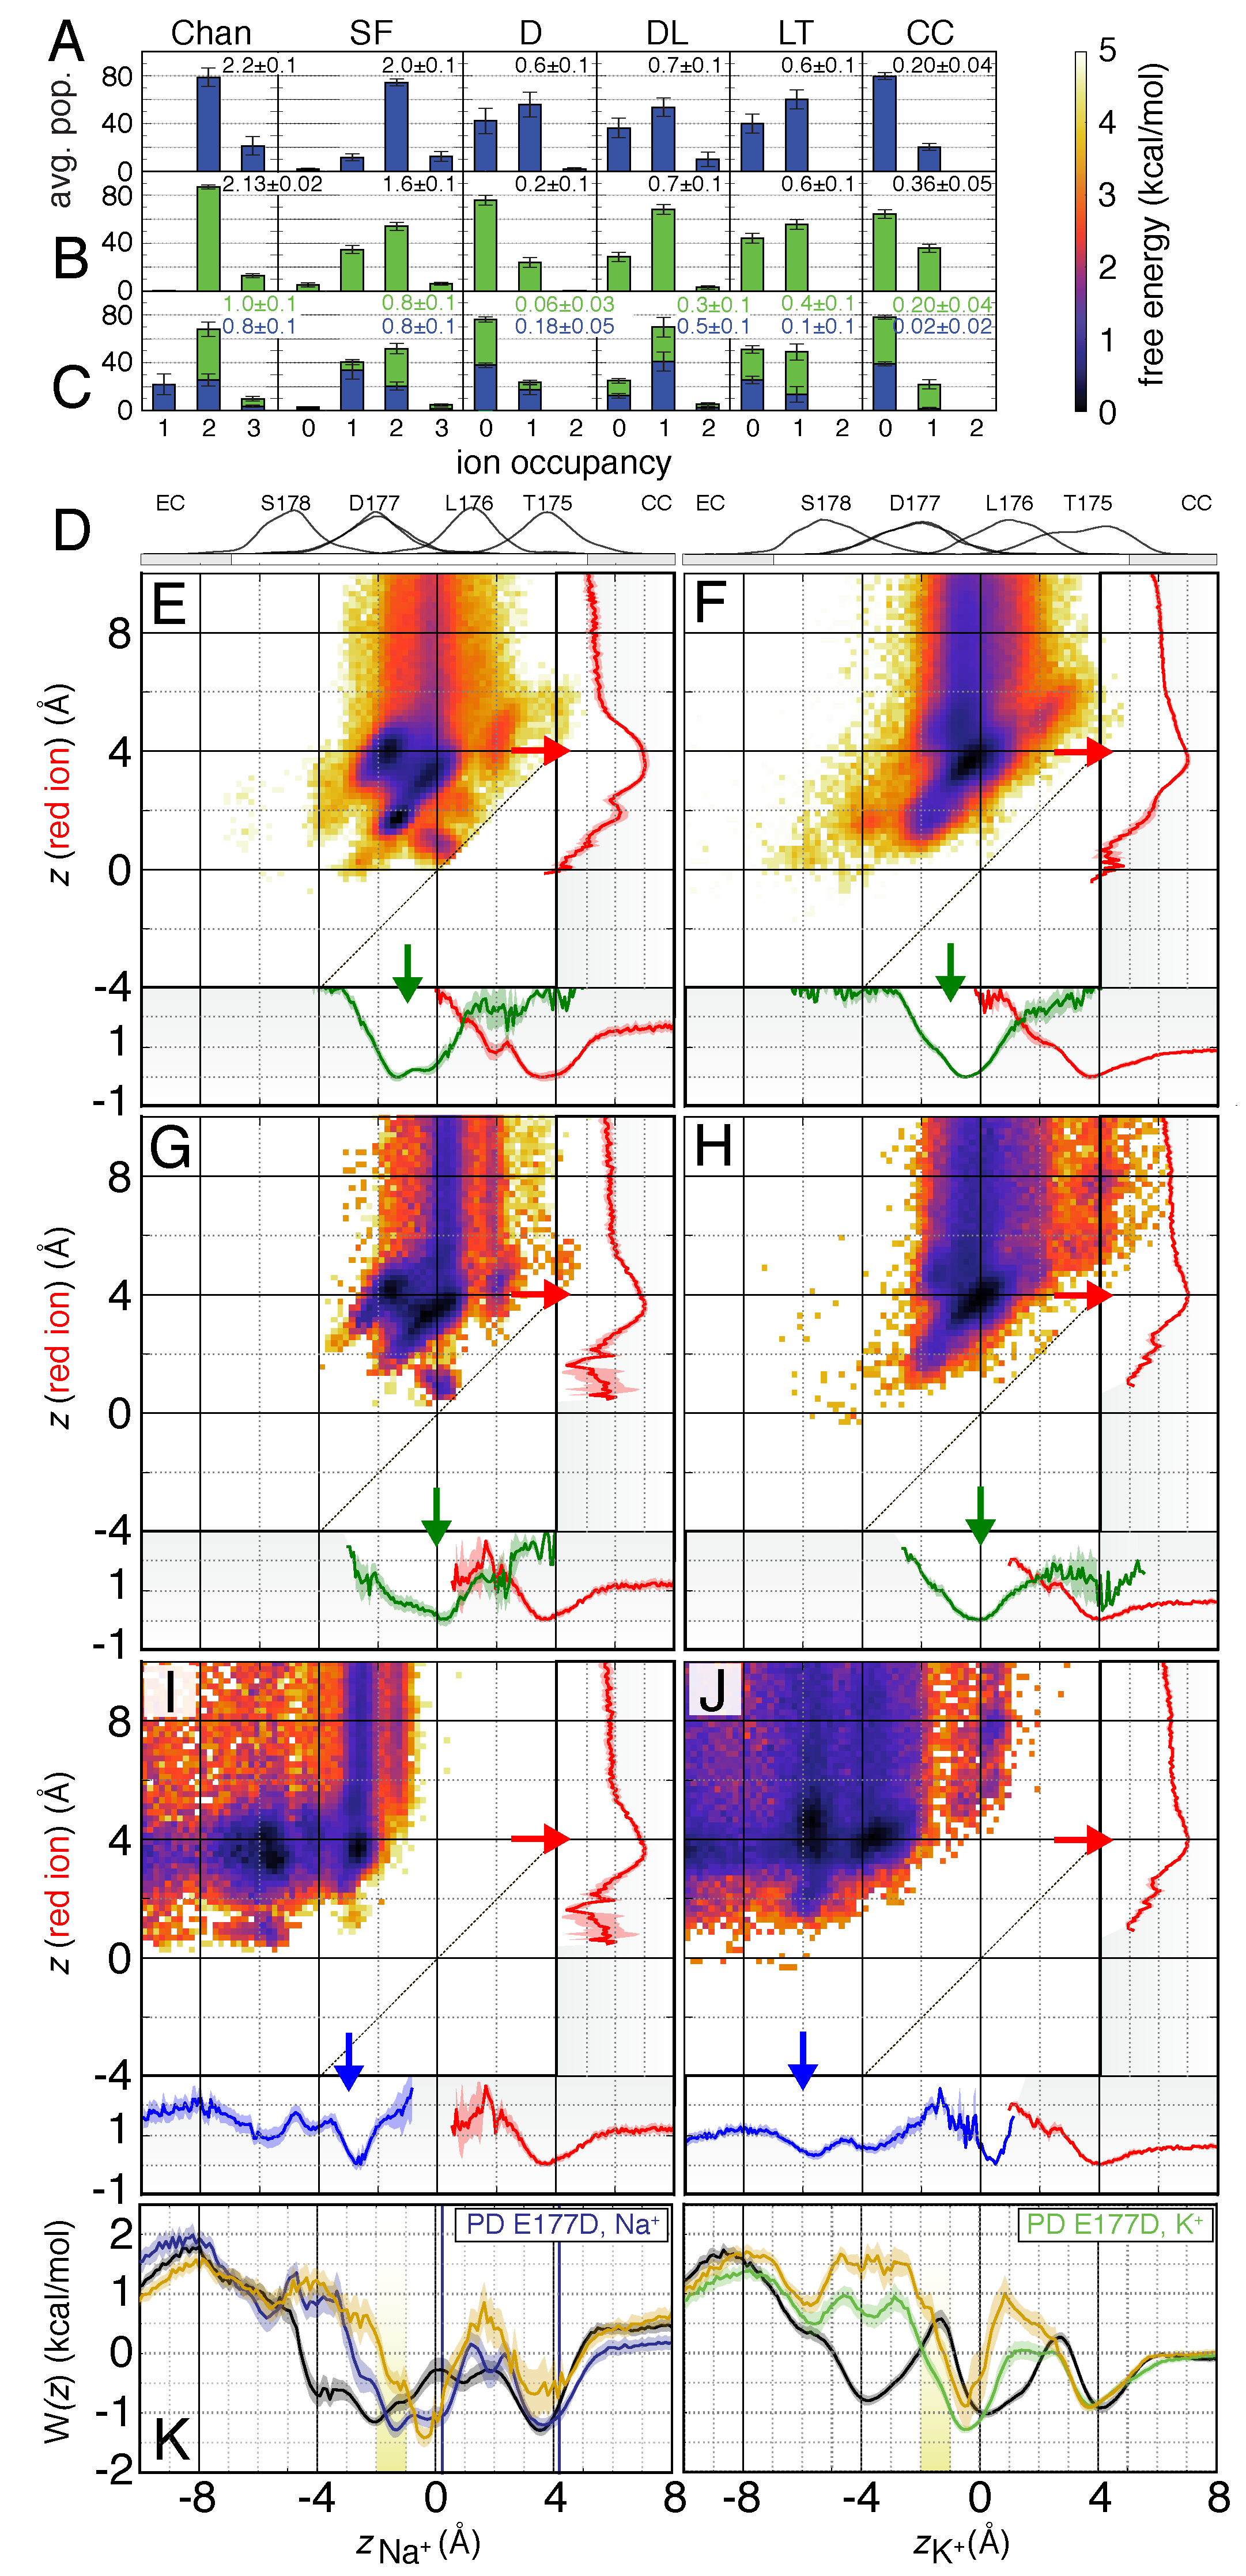
\includegraphics[width=0.6\textwidth]{nav2/Nav2Fig6}
\caption[Binding statistics and potential of mean-force (PMF) for the movement of Na$^+$ and K$^+$ along the channel axis in the E177D model]{\textbf{Binding statistics and potential of mean-force (PMF) for the movement of Na$^+$ and K$^+$ along the channel axis in the E177D model}. Ionic occupancy is shown from left to right for the entire channel, the SF, all major binding sites within the SF, together with the number of dunked E177 side chains, for (\textbf{A}) pure Na$^+$, (\textbf{B}) pure K$^+$, and (\textbf{C}) mixed cation simulations. (\textbf{D}) The axial distribution of pore-lining oxygen atoms of T175, L176, E177, and S178 for pure Na$^+$ and pure K$^+$ simulations. 2D PMFs for Na$^+$ and K$^+$ are computed between red and green ion pairs for the (E, F) 2 ion and (G,H) 3 ion occupancy state. 2D PMFs for (I) Na$^+$ and (J) K$^+$ are shown for the innermost and outermost ions, red and blue, respectively, for the 3 ion state. Multi-ion 1D projection onto the channel axis for pure (K) Na$^+$ and (L) K$^+$ (blue and green, respectively), with a black line showing the free energy of ion conduction for Na$^+$ and K$^+$ in the WT PD model as a reference. Na$^+$ and K$^+$ in mixed cation simulations are shown as a gold line in both panels.}
\label{fig:nav2fig6}
\end{figure}

\begin{figure}[!ptb]
\centering
\includegraphics[width=0.7\textwidth]{nav2/Nav2FigS6}
\caption[Conformational isomerization of residue 177 side chains]{\textbf{Conformational isomerization of residue 177 side chains}. 2D potential of mean force (PMF) for side chain torsions ($\chi_1$, $\chi_2$) of E177 with representative snapshots showing main conformers from each dataset. These conformers are rendered for two opposite subunits from the SF, corresponding to coloured circles labelled on the plots (purple, yellow, red, green). (\textbf{A}) Free energy profiles for ($\chi_1$, $\chi_2$) of E177 in the (left) PD+VSD and (middle) PD model in the presence of a mixture of Na$^+$ and K$^+$. 2D PMF plots for D177 side chain dihedral angles in the presence of pure Na$^+$ with a representative snapshot. Free energy profiles for ($\chi_1$, $\chi_2$) of E177 in the (\textbf{B}) HNNN model. In the HNNN model, the 2D PMF is calculated for subunit 1 (the protonated side chain, showing a representative snapshot) and subunits 2-4 (all deprotonated), in the presence of pure Na$^+$, as well as subunits 1-4 in the presence of pure K$^+$ (with the same protonation states). In-set boxes show the total percentage of data in two regions of $\chi_1$, $\chi_2$ space, corresponding to `undunked' and `dunked' conformations from top to bottom, separated by a dashed black line, in the WT and OPLS models. In the HNNN model, all boxes except the top left region represent a `dunked' conformation.}
\label{fig:nav2figS6}
\end{figure}

Simulations using a Na\textsubscript{V}Ab model with the sidechain shortening E177D mutation enable the study of ion conduction and selectivity under conditions where the diameter of the SF is effectively modified without changing the SF backbone. This mutation was found to reduce the Na$^+$:K$^+$ selectivity ratio to approximately 2:1 in the channel NaChBac \cite{FinolUrdaneta:2014bz}. E177D mutants crystallized of NavMs provided evidence that Na$^+$ binding may be eliminated in the outer binding site of the SF \cite{Naylor:2016cu}. In our simulations, the average channel occupancy for Na$^+$ and K$^+$ did not drop compared to WT models. However, the roughly balanced populations of the 2 and 3 ion states in the WT model shifted in favor of the 2 ion state for K$^+$ ($87\pm2$ and $13\pm2$\% for the 2 and 3 ion states, respectively) while Na$^+$ remained nearly unchanged ($76\pm8$ and $21\pm8$\% for the 2 and 3 ion states, respectively) (Fig. \ref{fig:nav2fig6} A,B). In both 2 and 3 ion states, the primary binding sites of the green and red ions are `DL' and `LT'. There is a significant loss of binding affinity at the `D' site (formerly `E', at -4 \AA) for the green ion (Fig. \ref{fig:nav2fig6} E-H, \ref{fig:nav2figS4} H,I), which is most pronounced for the green K$^+$, which no longer binds at the two sites (Fig. \ref{fig:nav2fig3} A-B). Reduction of D177-only binding occurs because the D177 sidechain is not long enough to  hold an upfacing conformation completely away from the channel lumen (where $\chi_2$ now refers to symmetric rotation about the C-C bond, Fig. \ref{fig:nav2figS6} B). Nonetheless, the previously described mechanisms of ion conduction are still possible for Na$^+$ and K$^+$ in pure cation E177D systems, with the exception that both the 2 and 3 ion states may support two Na$^+$ at the same axial position (at position $\sim$0 \AA). Specifically, the loosely knock-on mechanism in which 3 ion occupancy lowers the free energy barrier for the red ion to enter the `CC' holds also holds in the E177D mutant.
Na$^+$ and K$^+$ channel occupancy in mixed cation simulations are within error ($0.8\pm0.1$ and $1.0\pm0.1$, for Na$^+$ and K$^+$, respectively, Fig. \ref{fig:nav2fig6} C), in contrast with the marked preference for Na$^+$ over K$^+$ in the WT PD model ($1.6\pm0.1$ and $0.8\pm0.1$, for Na$^+$ and K$^+$ channel occupancy, Fig. 4H). As qualitatively compared using the 1D PMF, the primary features, namely well-depths and barrier heights, of the free energy profile are identical for Na$^+$ and K$^+$ conduction in pure and mixed cation simulations (Fig. \ref{fig:nav2fig6} I,J). Peak solvation of Na$^+$ and K$^+$ by carboxylate groups drops from $\sim$3 to $\sim$2 in this mutant (Fig. \ref{fig:nav2figS5} E,F). All ion pair 2D PMFs show that it is possible for Na$^+$ to pass itself in pure and mixed cation simulations, but it is never observed at the same axial position as K$^+$ in mixed cation simulations (Fig. \ref{fig:nav2figS7-5} F-J). Here we also show that there is no preferential binding of Na$^+$ or K$^+$ in mixed salt solutions. Our simulations show that the E177D mutation makes the channel non-selective by reducing K$^+$ binding affinity to the `D' site. 

\begin{figure}[!ptb]
\centering
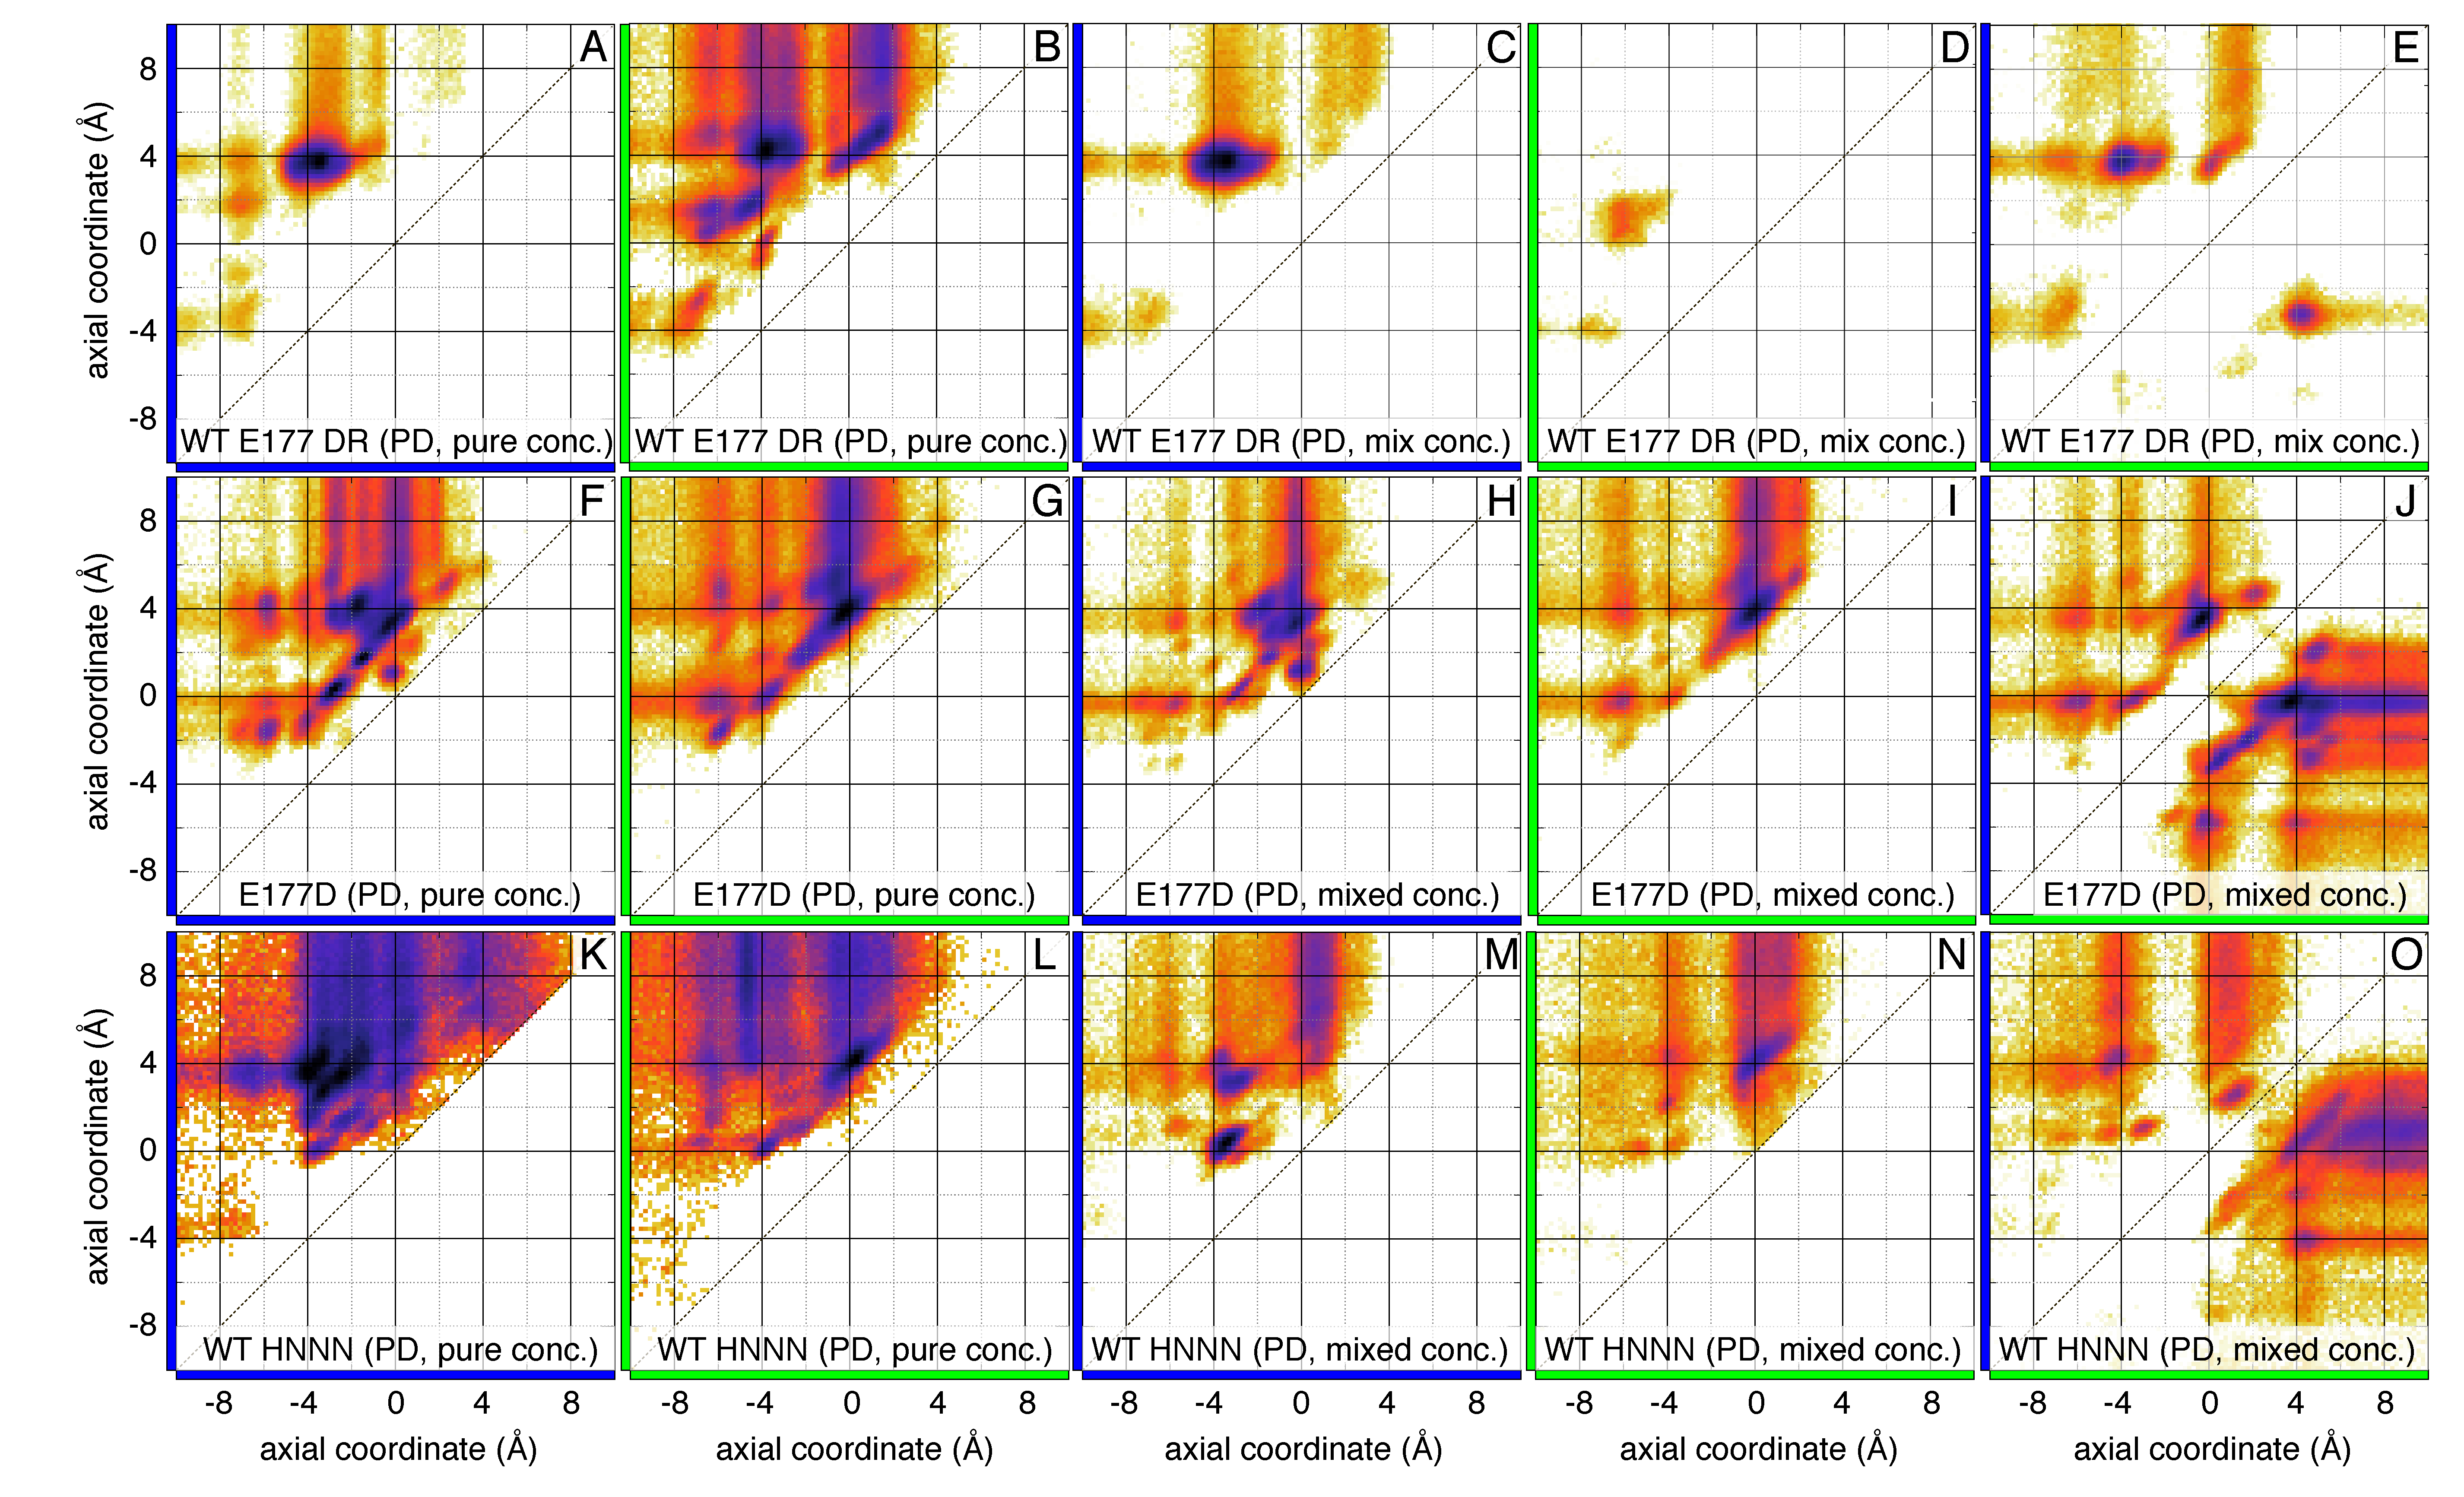
\includegraphics[width=0.7\textwidth]{nav2/Nav2FigS7-5}
\caption[Additional two-dimensional potential of mean-force (PMF) for Na$^+$ and K$^+$ pairs along the channel axis]{\textbf{Additional two-dimensional potential of mean-force (PMF) for Na$^+$ and K$^+$ pairs along the channel axis}. Ionic species are identified by a colored bar on the axes, Na$^+$ (blue) and K$^+$ (green). PMFs for (\textbf{A}) Na$^+$-Na$^+$ and (\textbf{B}) K$^+$-K$^+$ in pure cation simulations, and (\textbf{C-E}) Na$^+$-Na$^+$, K$^+$-K$^+$, and Na$^+$-K$^+$ in mixed cation simulations in the PD model with E177 dihedral restraints. (\textbf{F}) Na$^+$-Na$^+$ and (\textbf{G}) K$^+$-K$^+$ in pure cation simulations, and (\textbf{H-J}) Na$^+$-Na$^+$, K$^+$-K$^+$, and Na$^+$-K$^+$ in mixed cation simulations in the E177D model. (\textbf{K}) Na$^+$-Na$^+$ and (\textbf{L}) K$^+$-K$^+$ in pure cation simulations, and (\textbf{M-O}) Na$^+$-Na$^+$, K$^+$-K$^+$, and Na$^+$-K$^+$ in mixed cation simulations in the HNNN singly protonated E177 model. The reference state (zero free energy) is set to the high probability state for each pure cation or mixed cation simulation dataset, respectively.}
\label{fig:nav2figS7-5}
\end{figure}

\subsection{Effect of E177 protonation}

\begin{figure}[hp]
\centering
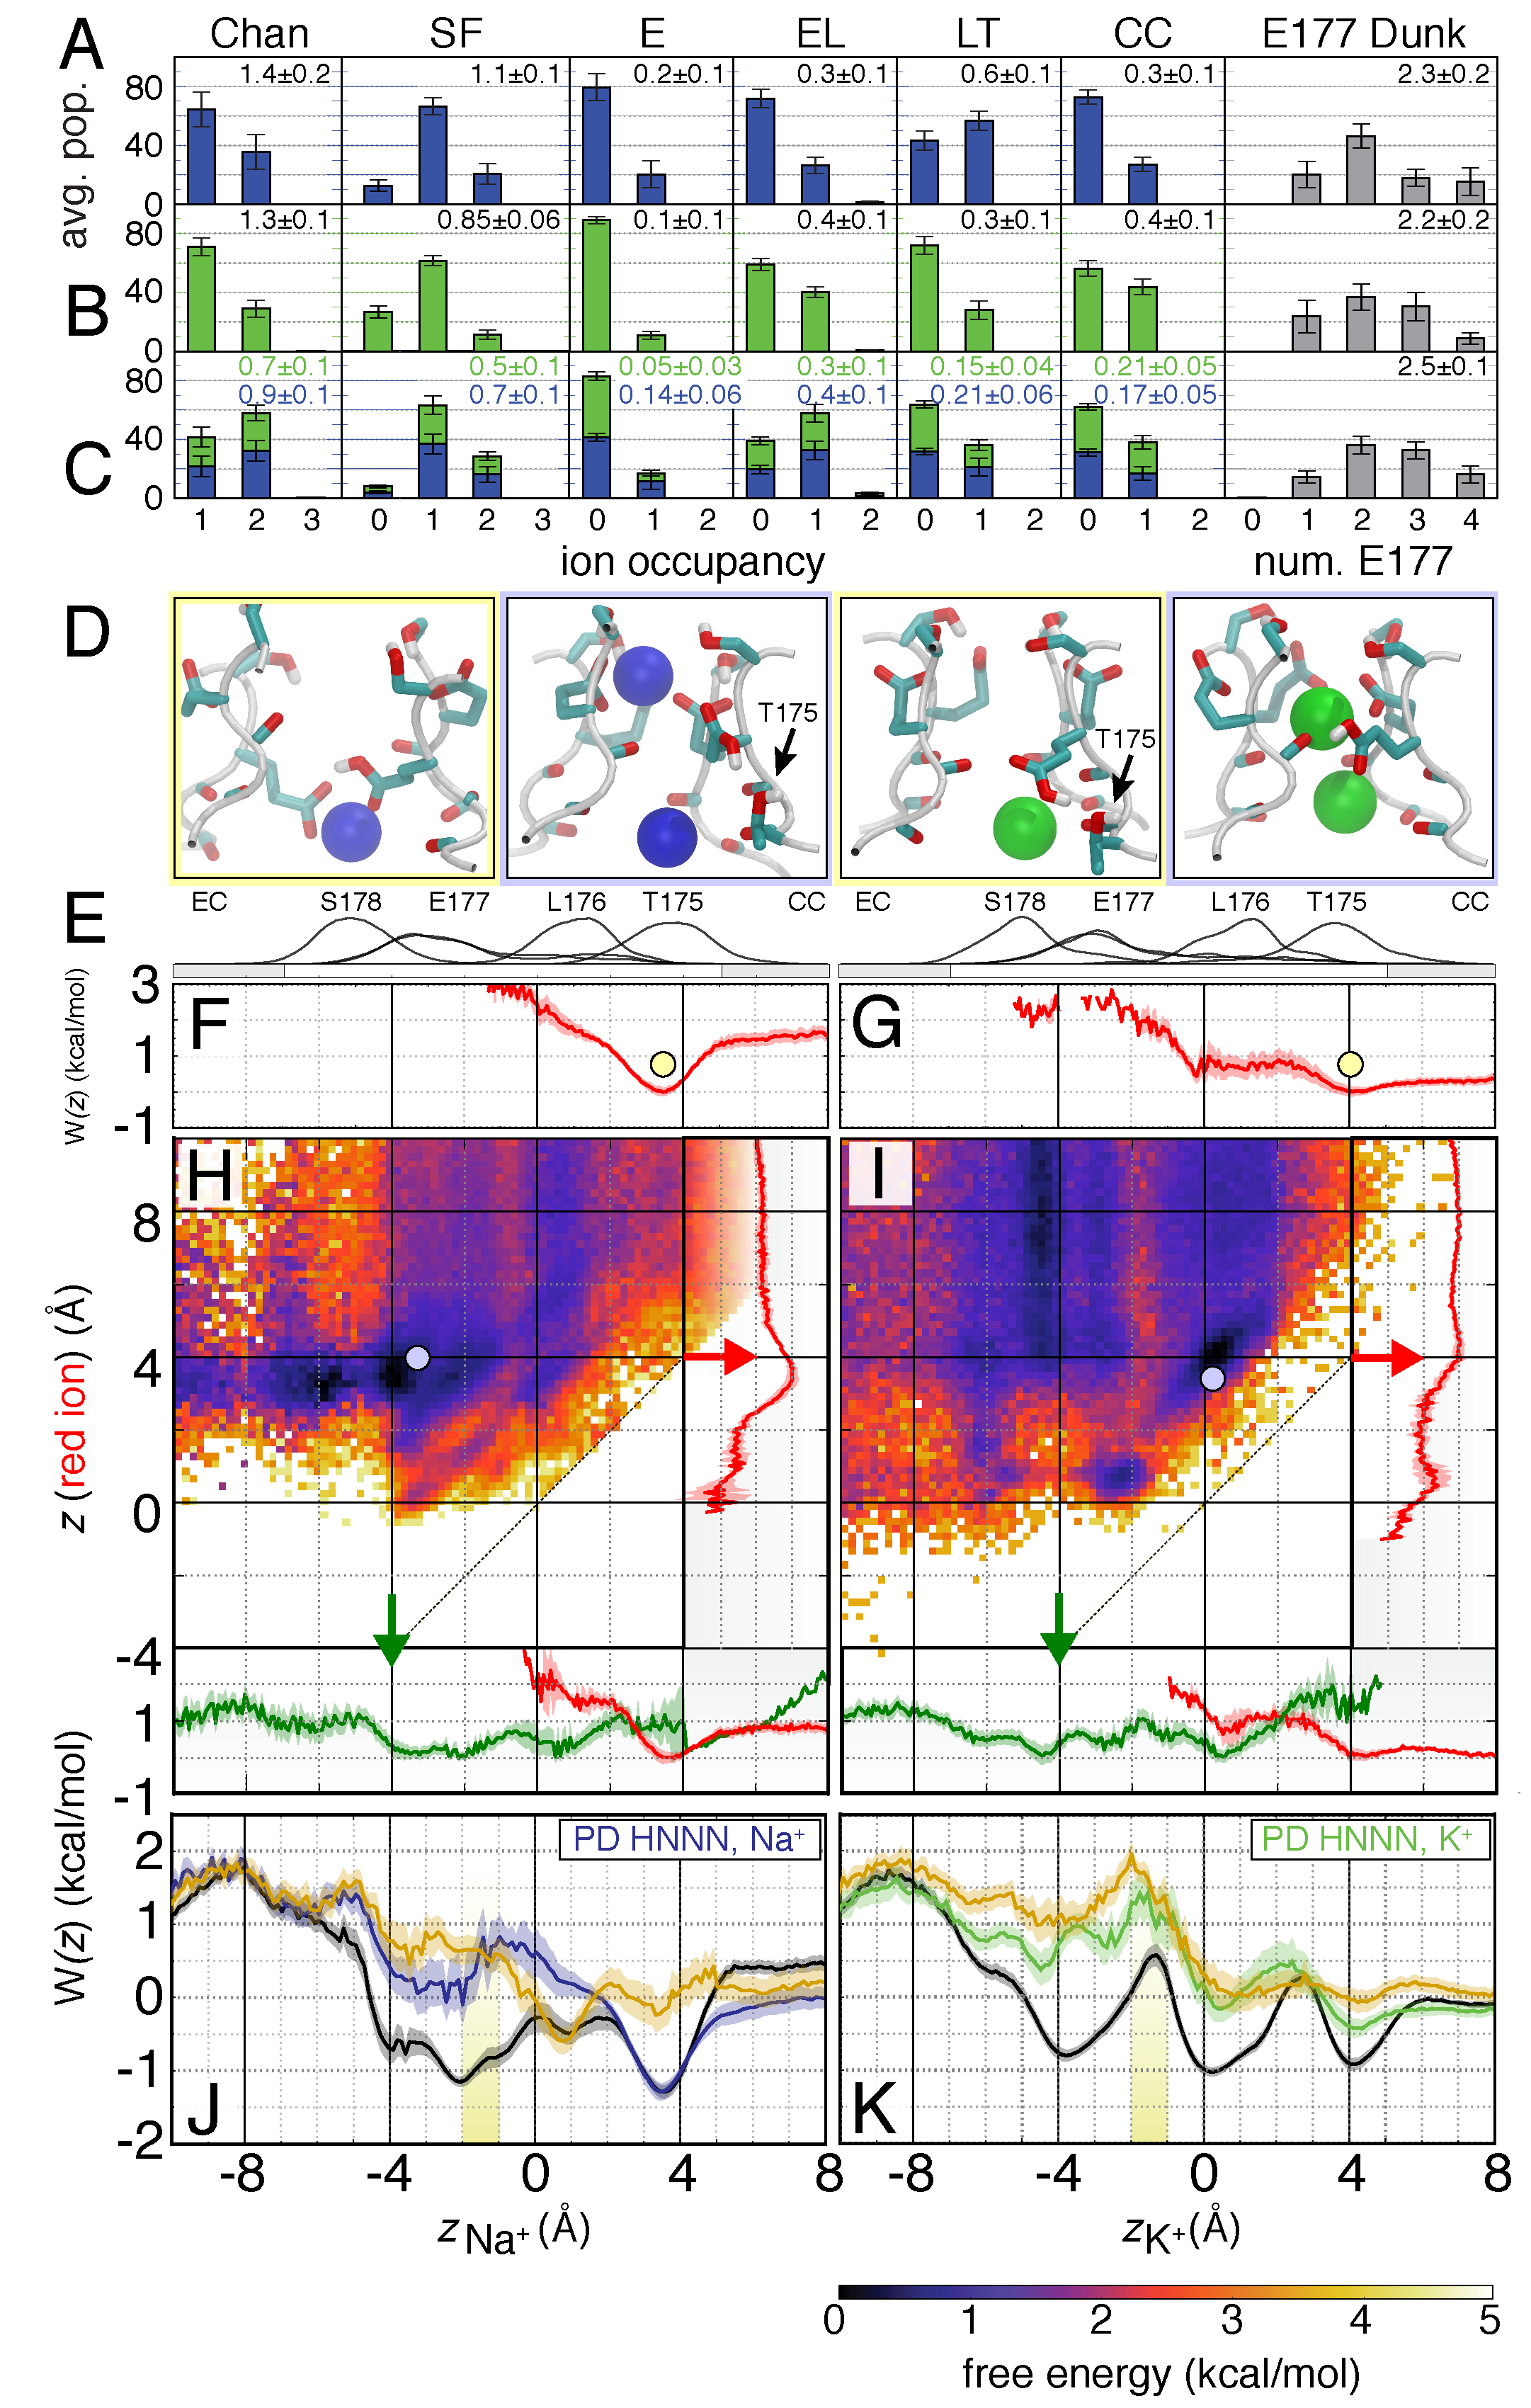
\includegraphics[width=0.6\textwidth]{nav2/Nav2Fig7}
\caption[Binding statistics and potential of mean-force (PMF) for the movement of Na$^+$ and K$^+$ along the channel axis in the single E177 protonated model]{\textbf{Binding statistics and potential of mean-force (PMF) for the movement of Na$^+$ and K$^+$ along the channel axis in the single E177 protonated model}. Ionic occupancy is shown from left to right for the entire channel, the SF, all major binding sites within the SF, together with the number of dunked E177 side chains, for (\textbf{A}) pure Na$^+$, (\textbf{B}) pure K$^+$, and (\textbf{C}) mixed cation simulations. (\textbf{D}) Representative snapshots of dominant ion configurations within the SF. (\textbf{E}) The axial distribution of pore-lining oxygen atoms of T175, L176, E177, and S178 for pure Na$^+$ and pure K$^+$ simulations. 1D PMFs for (\textbf{F}) Na$^+$ and (\textbf{G}) K$^+$ in the 1 ion occupancy state. 2D PMFs for Na$^+$ and K$^+$ are computed between red and green ion pairs for the (\textbf{H, I}) 2 ion occupancy state. Multi-ion 1D projection onto the channel axis for pure (\textbf{J}) Na$^+$ and (\textbf{K}) K$^+$ (blue and green, respectively), with a black line showing the free energy of ion conduction for Na$^+$ and K$^+$ in the WT PD model as a reference. Na$^+$ and K$^+$ in mixed cation simulations are shown as a gold line in both panels.}
\label{fig:nav2fig7}
\end{figure}

Experimental studies have shown that lowering the external pH from 7.4 to 5.8, presumably reducing the net anionic charge of the SF via protonation of one or more E177 side chains, results in a drop of Na$^+$ over K$^+$ selectivity from $\sim$33:1 to $\sim$7:1 in bacterial Na$^+$ channel NaChBac \cite{FinolUrdaneta:2014bz}. To test the influence of E177 protonation on cation permeation and selectivity, we performed simulations in which a single E177 sidechain was protonated. Protonation of the carboxylate group increased overall dunking affinity (Figs. \ref{fig:nav2fig7} A-C) and enabled the E177 side chain to adopt a large number of $\chi_1$,$\chi_2$ conformations unobserved in any other simulations, including those that permitted E177 coordination to ions bound in the `LT' binding site (Figs. \ref{fig:nav2fig7} D, \ref{fig:nav2figS6} C). Single E177 protonation resulted in a decrease of SF occupancy by $\sim$1 cation for both Na$^+$ and K$^+$ in pure cation simulations (Fig. \ref{fig:nav2fig7} A-B). Protonation decreases channel occupancy by $\sim$1 cation for Na$^+$ ($64\pm11$ and $32\pm11$\% for the 1 and 2 ion state populations, respectively) and K$^+$ ($71\pm6$ and $29\pm6$\% for the 1 and 2 ion state populations, respectively) (Fig. \ref{fig:nav2fig7} A,B). Binding of Na$^+$ and K$^+$ at `E' site is reduced by a factor of $\sim$4 and at the `EL' site by a factor of $\sim$2 when compared to the pure cation simulations in the PD system. In the 1 and 2 ion occupancy state, the red ion binds at the `LT'/`CC' site, where increased occupancy results in a lower free energy barrier to enter the `CC' for Na$^+$ (Fig. \ref{fig:nav2fig7} F-I). The green Na$^+$ and K$^+$ traverse a relatively flat free energy landscape wherein the entry of the red ion into the CC can occur at nearly any position (Fig. \ref{fig:nav2fig7} H-I). 
Although ion binding was reduced for both ions with respect to the fully deprotonated EEEE ring, the SF retained a small preference for Na$^+$ over K$^+$ in `E' and `EL' binding sites in mixed cation simulations. This minor preference for Na$^+$ over K$^+$ can be seen qualitatively in the 1D pseudo-PMF (Fig. \ref{fig:nav2fig7} H-I). Our simulations show that single E177 protonation reduces Na$^+$ selectivity over K$^+$.

\section{Discussion}

\subsection{Molecular Mechanism of Na$^+$ Selectivity}

The above results lead to four primary conclusions: 
\begin{itemize}
\item Na$^+$ and K$^+$ bind with similar stoichiometry in the SF of Na\textsubscript{V}Ab, with multiple binding modes involving a variable number of cations and a variable number of carboxylate groups of E177 side chains.
\item Conformational isomerization of E177 side chains is necessary to catalyze the conduction of Na$^+$ through the SF, whereas K$^+$ does not require E177 fluctuations to facilitate conduction. 
\item When the two types of cations compete with each other at equal concentrations, K$^+$ binding affinity is reduced at all SF binding sites in favor of Na$^+$. 
\item Selectivity for Na$^+$ originates from a difference in the multi-ion mechanism of ion translocation for Na$^+$ and K$^+$. 
\item Both side chain length reduction and reduction of anionic charge in the SF has the capacity to reduce binding affinity and selectivity for Na$^+$ over K$^+$.
\end{itemize}

The capability of the SF to provide a liquid-like free energy landscape for Na$^+$ but not for K$^+$ has its basis in the interaction between carboxylate side chains and the two ions. More effective coordination of Na$^+$ by E177 compared to K$^+$ is consistent with the concept of ionic field strength, whereby the carboxylate group is a classic high-field-strength ligand favoring the smaller cation, Na$^+$, over K$^+$ (difference in Pauling radii of 1.33 - 0.95 = 0.38 \AA) \cite{Eisenman:1962dy}.  Similarly, the preference for Na$^+$ over K$^+$ in the Na1 site of the LeuT transporter was recently ascribed to a carboxylate group from the leucine substrate \cite{Yu:2010dj} along the principle of the field-strength model.  A recent MD study of the SF of a mammalian NaV channel, in which the residues of the DEKA locus were inserted into the prokaryotic NaV channel, NaVRh, also attributed selection of Na$^+$ over K$^+$ ions in part to interactions with Asp and Glu side chains in the SF \cite{Xia:2013dv}. However, our analysis of average ionic coordination of Na$^+$ and K$^+$ within the SF shows that channel and water oxygen coordination of individual ions are not significantly different, and thus are unlikely to be the sole determinant for selectivity. Consistent variations in ion coordination between Na$^+$ and K$^+$ within the SF would support a previously proposed model for Na$^+$ selectivity \cite{Corry:2012ge}, but our results do not support this model. Likewise, even though we did not employ non-equilibrium methods, in competitive binding we do not observe evidence for K$^+$ block of Na$^+$ within the SF as described in a previous study \cite{Ngo:2016es}.  

Although the SF of Na\textsubscript{V}Ab is wider than that of K$^+$ channels in the absence of dunking \cite{Payandeh:2012ib}, conformational isomerization of the side chains of E177 in the confined environment of the SF creates a flexible binding site that appears to be well suited for the preferential binding of Na$^+$ relative to K$^+$. In particular, the SF supports multiple Na$^+$, often side-by-side, whereas this does not occur for K$^+$. At a physical level, this may still be due to the difference in ionic radius of the two ions, where K$^+$ is too large to fit into an ionic cluster coordinated by multiple E177 side chains. In turn, these results suggest that the conformational flexibility of the Glu side chains favors a loosely-coupled conduction mechanism, ultimately resulting in Na$^+$ selectivity.

\subsection{Model Limitations}

In our previous Nav channel simulation study \cite{Chakrabarti:2013kd}, we computed Na$^+$ conductance in a closed channel model, and found this to be on the same order of magnitude as experimental estimates (1-10 million ions/sec). These calculations were performed on the basis of identical relative free energy inside the central cavity versus the bulk, no evidence for interactions between the SF and the contents of the CC, and the assumption that crossing the IC gate would occur faster than crossing the SF in an open channel. In the current pure and mixed simulation datasets presented in this work, we no longer have equal affinity for ions in the central cavity and the SF and `LT'/`CC' sites are never occupied simultaneously (Fig. \ref{fig:nav2fig2} B-C,  \ref{fig:nav2fig4} H), confirming that `CC' occupancy influences SF binding. However, the `CC' occupancy in our simulations (0.2-0.3 with a bulk ionic concentration of 247 mM, Fig. \ref{fig:nav2fig2} B), was comparable to the CC occupancy of an open K$^+$ channel (0.24 with a bulk K$^+$ concentration of 140 mM) \cite{Sumikama:2016kb}, suggesting that our simulations of the closed-state may still recover the binding affinity of the `CC' in the open-state. Regardless of `CC' occupancy, we determined several qualitative features, robust to simulation force field, which support a molecular mechanism for $\sim$2-fold selectivity of Na$^+$ over K$^+$. These findings, particularly those pertaining to the role of glutamic acid side chains in selectivity, are unlikely to be altered in a model of the open-state channel given that the open-state SF is unchanged from the closed-state structure used in our simulations. 

\subsection{Comparison to Previous Computational and Experimental Studies}
Even though electron density corresponding to Na$^+$ was not identified within the SF of the Na\textsubscript{V}Ab I217C structure used in this study \cite{Payandeh:2012ib}, three highly occupied Na$^+$ binding sites were observed in the SF of a homologous 2.7 \AA NavMs structure \cite{Naylor:2016cu}. These binding sites correspond roughly to positions of the proposed S$_{HFS}$, S$_{CEN}$, and $S_{IN}$ sites. Previous simulation studies disagree on the number of binding sites within the SF, reporting two \cite{Chakrabarti:2013kd,Furini:2012jl}, three \cite{Boiteux:2014ut,Corry:2012ge}, four \cite{Domene:2015kj,Ke:2014fy}, or five Na$^+$ binding sites \cite{Stock:2013cg,Ulmschneider:2013da}, which also differ in axial position. In this work, we identified three primary Na$^+$ binding sites defined by ionic coordination to residues `E', `EL', and `LT' (Fig. \ref{fig:nav2figS4}). These sites are in qualitative agreement with the binding sites observed in the NavMs SF \cite{Naylor:2016cu}. 

Accurate simulations of a bacterial Nav channel should reproduce electrophysiological conductance (1-10 million ions/sec) and selectivity measurements ($\sim$10:1 Na$^+$ over K$^+$). Even for well-studied channels, such as gramicidin and KcsA, simulations underestimate experimental conductance \cite{Allen:2004vs,Jensen:2013gn}. Although the calculated conductance and selectivity from one NavMs channel simulation study were on the correct order of magnitude for Na$^+$ and K$^+$ \cite{Ulmschneider:2013da}, our work challenges several findings from this manuscript. In our simulations with E177 restrained in the crystallographic conformation, we observed greatly reduced binding at the `EL' site, resulting in an axial distribution of ions very similar to the one presented in that work \cite{Ulmschneider:2013da}. These discrepancies must be due to methodological differences between our study and Ulmschneider et al., namely; an open-state pore-domain model, structural restraints, and external applied voltage. However, a systematic study is required in order to pin point the source of this discrepancy. 

Our understanding of selectivity in Nav channels is further strengthened by examining SF modifications that reduce Na$^+$ selectivity. Results from E177D simulations indicate that both the binding affinity and the conduction mechanism are similar for Na$^+$ and K$^+$ in pure and mixed cation models, in a manner consistent with electrophysiological and computational studies showing that the E177D mutant is poorly selective \cite{FinolUrdaneta:2014bz}. Our simulations in pure and mixed cation E177 protonated models are also consistent with the decrease in Na$^+$:K$^+$ selectivity measured in the same study \cite{FinolUrdaneta:2014bz}. Pure cation simulations of Na$^+$ in this model are in agreement with previous PMF calculations showing changes in E177 conformational isomerization and a large decrease in binding at the `E' site of the channel \cite{Furini:2014gv}. Inversely, our results do not agree with an unbiased equilibrium simulation reporting that the singly-protonated SF had a comparable free energy of Na$^+$ conduction to the fully charged EEEE ring  \cite{Boiteux:2014ut}.

Future calculations of conductance in a stable open-state Nav channel structure may assist in better understanding the role of channel fluctuations (in the SF and TM regions), multi-ion effects, and voltage on conductance and selectivity. Such studies should provide complimentary information to the mechanistic description of ion movement through the SF in pure and mixed cation concentrations, potentially reweighting the populations of states observed within the SF in our simulations to offer a more complete picture of Na$^+$ selectivity.

\section{Methods} 

\subsection{Molecular Modelling and Simulation} 

Multiple all-atom molecular models were constructed using the Na\textsubscript{V}Ab I217C structure (PDB code: 3RVY) \cite{Payandeh:2012ib} (Fig. S1). The three models employed in this study (named PD, PD+VSD, and OPLS PD+VSD), with the exception of the voltage sensor domains, differ primarily in the size of the simulation cell. %A summary of all molecular models and simulation datasets are presented in Table S1.

In the PD+VSD model, all transmembrane domains of the Na\textsubscript{V}Ab I217C structure (S1-S6, residue 1-221) were embedded in a hydrated 1,2-dimyristoyl-sn-glycero-3-phosphatidylcholine (DMPC) bilayer (270 lipid molecules) with a NaCl or KCl concentration of 247 mM. Both N- and C-terminal ends of the protein were modeled as neutral moieties. This simulation cell was comprised of $\sim$129,000 atoms with approximate dimensions of 10.8 $\times$ 10.8 $\times$ 11.3 $nm^3$. Membrane embedding was performed using alchembed \cite{Jefferys:2015jt} with an equilibrated CHARMM36 DMPC bilayer patch obtained from the Jeffery Klauda laboratory website (https://terpconnect.umd.edu/$\sim$jbklauda/research/download.html). The protein, lipids, and ions were modeled with the CHARMM36 all-atom force field \cite{Best:2012kb,Best:2012uu,MacKerell:1998tp,Klauda:2010tn}, and water molecules were modelled with TIP3P \cite{Jorgensen:1983ty}. NBFIX adjustments were made for Na$^+$ - backbone carbonyl oxygen atom interactions \cite{Noskov:2008jp}, as well as NBFIX corrections for Na$^+$ - lipid head group interactions \cite{Venable:2013ix} (note that equivalent Na$^+$ - protein carboxylate group interactions were not used since not equivalent parameterization was available for K$^+$). 

All PD+VSD and PD simulations were performed with GROMACS 4.6.5 \cite{Hess:2008db} using the same simulation settings. Electrostatic interactions were calculated using particle-mesh Ewald \cite{Essmann:1995vj,Darden:1993vu} with a real-space cut-off distance of 1.2 nm, a grid spacing of 0.16 nm, and cubic interpolation. Lennard-Jones interactions were cut off at 1.2 nm. Nonbonded interactions were calculated using Verlet neighbor lists \cite{Verlet:1967cm}. All simulations were performed at constant temperature (300 K) and pressure (1 atm) using the Nos\'e-Hoover thermostat \cite{Hoover:1985wf,Nose:1984em} with temperature coupling of 0.5 ps and the Parrinello-Rahman barostat \cite{Nose:1983cu,Parrinello:1980uc} with a time constant of 2 ps, respectively. All chemical bonds were constrained using the LINCS algorithm \cite{Hess:2008fl}. The integration time step was 2 fs. 

For both NaCl and KCl concentrations, steepest descent minimization was used to ensure forces less than 1000 kJ mol$^{-1}$ nm$^{-2}$, followed by three successive NPT simulations of 10ns to assist in equilibration. In these equilibration steps, position restraints were applied to heavy atoms, main chain backbone atoms, and then C$\alpha$ atoms, with restraint strength of 1000 kJ mol$^{-1}$ nm$^{-2}$. Fifteen simulation repeats were then generated with randomized initial velocities for both NaCl and KCl concentrations, and run for 1,000 ns. Across both NaCl and KCl, an aggregate total of 30 $\mu$s was performed using the PD+VSD model.

In the PD model, the pore domain of Na\textsubscript{V}Ab (S5-S6, residue 130-221) was embedded in a hydrated DMPC bilayer with a salt concentration of 240 mM. Both N- and C-terminal ends of the protein were modeled as neutral moieties. A hydrated DMPC lipid patch of 200 lipids in 150mM NaCl was generated using CHARMM-GUI \cite{Wu:2014uc} and equilibrated under NPT for 20 ns with the CHARMM36 force field \cite{Klauda:2010tn}. Membrane embedding was performed using g_membed \cite{Wolf:2010dr} where 14 lipid molecules were removed. This resulted in a periodic rectangular cell comprised of $\sim$61,000 atoms with approximate dimensions of 8.3 $\times$ 8.3 $\times$ 8.3 nm$^3$. In mixed cation simulations of the PD model, the salt concentration was 197 mM for both NaCl and KCl. Using the identical pure and mixed cation models, additional systems were constructed with modifications made to the EEEE ring, including the E177D mutation and the protonation of a single E177 side chain. The protein, lipids, and ions were modeled with the CHARMM36 all-atom force field \cite{Best:2012kb,Best:2012uu,MacKerell:1998tp,Klauda:2010tn}, and water molecules were modelled with TIP3P \cite{Jorgensen:1983ty}, identical to the parameters used for PD+VSD simulations above.

An alternative PD+VSD model was used in simulations of the OPLS force field \cite{Jorgensen:1996vx,Kaminski:2001eq}. This system has a larger simulation cell comprised of $\sim$219,000 atoms in total, with approximate dimensions of 16.7 $\times$ 16.7 $\times$ 9.8 nm$^3$. The OPLS NaCl dataset used in this work is identical to the one utilized in our previous manuscript \cite{Chakrabarti:2013kd}, and we generated a new OPLS KCl dataset using an identical modelling and simulation protocol. In this system, the protein was modeled with the OPLS-AA/L all-atom force field \cite{Jorgensen:1996vx,Kaminski:2001eq} with default ions parameters \cite{Aqvist:1990ud}, the lipid bilayer was modelled with Berger parameters \cite{Berger:1997bc}, and water was modelled with the TIP3P model \cite{Jorgensen:1983ty}. 

Forty-seven simulations of 400-500 ns each as well as forty-eight 500-ns simulations yielded 21.6 and 24 $\mu$s of simulation data for NaCl and KCl simulations. A set of ten 250 ns NaCl simulations was performed using the same OPLS NaCl model with the addition of E177 side chain dihedral restraints, ($\chi_1$,$\chi_2$) = (210 degrees, 290 degrees), with a force constant of 5000 kJ mol$^{-1}$ rad$^{-2}$. Simulations were performed with GROMACS 4.0.7 \cite{Hess:2008db}. 

Mixed cation simulations in the OPLS PD+VSD model were performed in two stages, where only the latter stage is presented in this study. With equal concentrations of 150mM NaCl and 150 mM KCl, we observed that systematic errors in the ion parameters of the OPLS forcefield resulted in significant Na$^+$ binding to the lipid head group region. This resulted in a decrease of bulk ionic concentration of Na$^+$ from an expected 150mM to approximately 90mM. Bulk ion concentration of K$^+$ in competition studies was also larger than 150mM at approximately 190mM. Due to the importance of equal sodium and potassium for competitive binding studies, we performed fifty additional competition simulations of 300ns (15 $\mu$s) where this bias was corrected. Initial conditions for these corrected concentration runs were carefully selected in order to reproduce the expected populations of the EL, E, and CC binding sites we would expect for the equal Na$^+$ and K$^+$ concentrations (approximately double the sodium binding propensity). Specifically, twenty-five initial conditions were selected from a pool of the forty-five final frames of the first set of competition runs (at approximately t=500ns). Initial conditions were randomly selected from the pool until the ratios of ionic occupancy across the ensemble (E 12:1, EL 2.5:1, CC 0.35:1) were twice that of the original competition runs (E 5.4:1, EL 1.25:1, CC 0.28:1). Water oxygens in a region outside of 30 \AA from the protein were stochastically replaced with 55 Na$^+$ atoms. Additionally, 32 K$^+$ atoms were removed to correct for the overestimate of potassium concentrations. Two replicas for each initial condition were run with differing initial velocities and identical simulation parameters to the previous runs. Significant ion binding to the surface of the bilayer was not observed with the other force fields used in this study.

\subsection{Analysis} 
Atomic positions, ionic coordination, and dihedral angles of E177 side-chains were extracted using MDAnalysis \cite{MichaudAgrawal:2011fd}. All axial positions of ions were measured relative to the center of mass of the C$\alpha$ atoms of residues 175 and 178 for all subunits at each frame (a point approximately at the center of the selectivity filter). The position and coordination of all ions within a cylinder of radius 10 \AA (with arbitrary height) was centered at the SF center of mass. To correct for tilting of the protein within the bilayer, the principal axis of all protein atoms was computed at each frame and the positions of all atoms were projected onto this axis. 
The first-shell coordination of Na$^+$ or K$^+$ were computed by counting the number of oxygen atoms within 3.0 \AA or 3.4 \AA of the ions, respectively (corresponding to the first minima in the ion-protein oxygen radial distribution function). Second-shell coordination was computed by counting the number of occurrences of a water oxygen within 3.3 \AA of a channel oxygen while having same water oxygen within 3.0 \AA or 3.4 \AA of the Na$^+$ or K$^+$, respectively, while ensuring that the cation to channel oxygen distance was larger than both of the previous two distances (this count was also checked to remove cases of double counting). 
In the analysis of channel occupancy macrostates, the total channel occupancy was defined as the count of all ions within the axial range -10 \AA to 14 \AA. Macrostate populations were not sensitive to this axial cutoff value at the `EC' or `CC' boundaries. Similarly, a removal of `EC' ions from the total channel occupancy count was not found to have a significant effect on macrostate populations or kinetics.
In binding statistics analysis, channel occupancy was defined as the count of all ions within the axial range -10 \AA to 14 \AA (inherently within a 10 \AA radius cylinder centered within the SF). We utilized first and second shell coordination to define SF occupancy as any ion bound in the `E', `EL', or `LT' binding sites. Based on first shell and second shell coordination, each ion was labelled with a respective SF binding site. Failing to find a binding site, meaning no first shell coordination, ions were classified as `EC' or `CC' based on axial position (cutoffs of -5 \AA for `EC', and 5 \AA for `CC', but populations of these states were largely insensitive to these values). S178-only coordination of ions did not occur significantly in our dataset, and the remaining S178 and E177 coordinated ions were grouped into the `E' binding site. Given the high number of degenerate binding modes within the SF of Na\textsubscript{V}Ab, numerous binding modes of ions had to be manually grouped into a site based on their dominant first-shell channel ligands and sometimes ion axial position. In the case of OPLS simulations, the `LT' binding mode could be identified based on first shell coordination only, but in all other simulations, second shell coordination was needed to define this site. 
Potentials of mean force (PMF) were computed from axial ionic distributions $\rho$(z) using the following relationship: W(z) = -k$_B$T ln $\rho$(z), where k$_B$ and T are the Boltzmann constant and the absolute temperature, respectively. Similarly, 2D PMF maps were computed from the axial ionic distributions $\rho$(z$_1$, z$_2$) of distinct ion pairs (red/green, green/blue, red/blue), or all unique ion pairs using the following relationship: W(z$_1$, z$_2$) = -k$_B$T ln $\rho$(z$_1$, z$_2$), where we ensures that z$_1$ <  z$_2$. For example, in cases of triple ionic occupancy of the channel, all-pair plots simultaneously show the free energy of red-green, green-blue, and red-blue ionic configurations (Fig. \ref{fig:nav2figS7}).
E177 side chain dihedral angles are defined as $\chi_1$ = N-C$_{\alpha}$-C$_{\beta}$-C$_{\gamma}$ and $\chi_2$ = C$_{\alpha}$-C$_{\beta}$-C$_{\gamma}$-C$_{\delta}$. The dihedral angle values from our previous work were transformed by multiplying by -1.0 and adding 360 degrees if the value was less than 0.0 \cite{Chakrabarti:2013kd}. In this work we have not multiplied the initial angles by -1. 

All time averaged properties in this manuscript were computed with data recorded at a 20 ps intervals with the exception of the PD+VSD OPLS NaCl model that was recorded at 25 ps. Equilibration time, defined as the time needed to reach stable occupancy of the channel, is taken to be 150 ns for the pure and mixed cation systems selected. This is with exception to OPLS PD+VSD mixed cation simulations where no data was removed. In this system, mixed cation simulation repeats were equilibrated for 500ns. This equilibration period was removed prior to all analysis conducted in this work. All error bars in this manuscript were computed with the standard error of mean over all simulation repeats in a given simulation set, unless otherwise specified. The average oxygen coordination in Fig. \ref{fig:nav2figS5} was computed individually over all coordination values found in an axial histogram bin. Since many replicas did not sample all positions along the channel axis, positions not sampled would otherwise lower the estimate of ion coordination. 
In the case of 1D PMF calculations, we computed error bars using the following protocol. A unnormalized histogram of ionic positions was computed with 0.11 \AA spacing for each simulation repeat. Each histogram was normalized by the number of data points in that repeat (the same value within a simulation dataset in all our calculations except for OPLS PD+VSD NaCl). Very low non-zero counts in position histograms were found to introduce a large amount of error in the average and error, so positions with less than 3 data points were flagged and replaced with NaN values for exclusion from averaging. Each PMF was shifted such that its mean bulk value in the position range -20 \AA to -19 \AA (in the extracellular bulk) was set to a free energy of zero. The mean and standard error of mean for each PMF bin was then computed and used for plotting. In 2D PMF calculations, we only report the average over all simulation repeats and error is not shown. In these plots, the reference state (zero free energy) is set to the highest probability state for each pure cation or mixed cation simulation dataset, respectively, rather than the mean bulk value.
 
%\section{Supplemental Figures} 
%\beginsupplement









%\begin{figure}[!ptb]
%\centering
%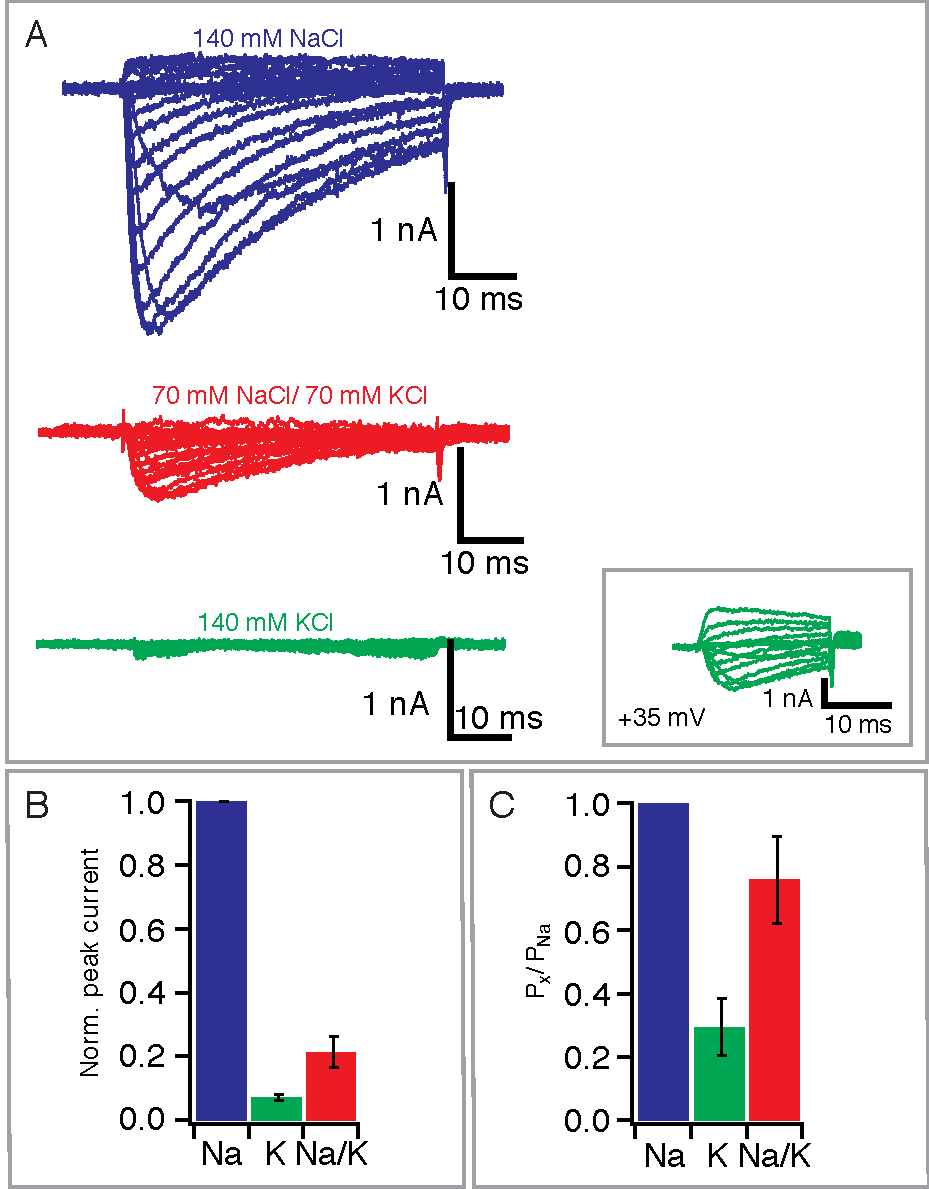
\includegraphics[width=0.7\textwidth]{nav2/Nav2FigS10}
%\caption[Na\textsubscript{V}Ab relative permeabilities measured with respect to intracellular solution containing 35 mM KCl and 105 CsF]{\textbf{Na\textsubscript{V}Ab relative permeabilities measured with respect to intracellular solution containing 35 mM KCl and 105 CsF}. (\textbf{A}) Whole cell currents using different extracellular solutions; 140 mM NaCl, 70 mM NaCl /70 mM KCl, and 140 mM KCl measured in the same cell showing the different sizes of inward currents. K$^+$ conductance was very low compared to Na$^+$ conductance or a mixture of Na$^+$ and K$^+$. Clear inward K currents were observed but only under conditions where the amount of channel expression was increased to extremely high levels (inset). (\textbf{B}) Mean peak current obtained with different extracellular solutions. (\textbf{C}) Relative permeabilities calculated from reversal potentials measured from IV curves.}
%\label{fig:nav2figS10}
%\end{figure}

\printbibliography[heading=subbibnumbered,title={References}]
\end{refsection}
\pagebreak
